\PassOptionsToPackage{unicode=true}{hyperref} % options for packages loaded elsewhere
\PassOptionsToPackage{hyphens}{url}
%
\documentclass[]{article}
\usepackage{lmodern}
\usepackage{threeparttable}
\usepackage{geometry}
\usepackage{amssymb,amsmath}
\usepackage{ifxetex,ifluatex}
\usepackage{fixltx2e} % provides \textsubscript
\usepackage{hyperref}
\usepackage{graphicx,grffile}
\usepackage{tabularx}
\usepackage{longtable}
\usepackage{paralist}
\usepackage{rotating}
\usepackage{ltxtable}

\usepackage{lscape}
\usepackage{booktabs, multirow} % for borders and merged ranges
\usepackage{soul}% for underlines
\usepackage[table]{xcolor} % for cell colors
\usepackage{changepage,threeparttable} % for wide tables
\usepackage{cite}

\ifnum 0\ifxetex 1\fi\ifluatex 1\fi=0 % if pdftex
\usepackage[T1]{fontenc}
\usepackage[utf8]{inputenc}
\usepackage{textcomp} % provides euro and other symbols
\else % if luatex or xelatex
\usepackage{unicode-math}
\defaultfontfeatures{Ligatures=TeX,Scale=MatchLowercase}
\fi

% use upquote if available, for straight quotes in verbatim environments
\IfFileExists{upquote.sty}{\usepackage{upquote}}{}
% use microtype if available
\IfFileExists{microtype.sty}{%
	
	\usepackage[]{microtype}
	\UseMicrotypeSet[protrusion]{basicmath} % disable protrusion for tt fonts
}{}

\IfFileExists{parskip.sty}{%
	\usepackage{parskip}
}{% else
	\setlength{\parindent}{0pt}
	\setlength{\parskip}{6pt plus 2pt minus 1pt}
}

\hypersetup{
	pdfborder={0 0 0},
	breaklinks=true}
\urlstyle{same}  % don't use monospace font for urls
\setlength{\emergencystretch}{3em}  % prevent overfull lines
\providecommand{\tightlist}{%
	\setlength{\itemsep}{0pt}\setlength{\parskip}{0pt}}
\setcounter{secnumdepth}{0}
% Redefines (sub)paragraphs to behave more like sections
\ifx\paragraph\undefined\else
\let\oldparagraph\paragraph
\renewcommand{\paragraph}[1]{\oldparagraph{#1}\mbox{}}
\fi
\ifx\subparagraph\undefined\else
\let\oldsubparagraph\subparagraph
\renewcommand{\subparagraph}[1]{\oldsubparagraph{#1}\mbox{}}
\fi

\renewcommand{\baselinestretch}{1.75}

\renewcommand{\arraystretch}{5}


\newgeometry{vmargin={15mm}, hmargin={30mm,30mm}}   % set the margins 


% set default figure placement to htbp
\makeatletter
\def\fps@figure{htbp}
\makeatother


\newcommand{\pplfont}[1]{{\textbf{\fontfamily{ppl}\selectfont #1}}}

\newcommand{\lmttfont}[1]{{\fontfamily{lmtt}\selectfont #1}}

\begin{document}

\section{Introduction}\label{introduction}

So far, we proved that semantic segmentation of liver tissues can be
performed using DL through robust CV training on both 3DIrcad-dB and
TheraHCC-dB.

We also demonstrated that both a cascaded architecture and the use of
multiphase information allows a better segmentation accuracy than using
single phases images only.

One of the main goals of our research work was to use imaging features
to predict pathological behavior of the disease. The prediction of the
histological grade of the tumor was rarely studied, since only one study
used deep learning tools to perform this task but with MR images as
input
(\href{https://www.hindawi.com/journals/bmri/2019/9783106/}{\emph{link}}).
Indeed, this task appears to be more challenging than previous DLR
liver-related work where either the type of FFL or the treatment
response (such as the recurrence) were predicted (see DLR section).

\section{Histological HCC grade in the literature
}\label{histological-hcc-grade-in-the-literature}

\subsection{Histological HCC grading
systems}\label{histological-hcc-grading-systems}

Several types of histological grading systems exist, with the most
frequent ones being ES 1954 and WHO 2010. Differences between those two
grading systems are given in the following table.

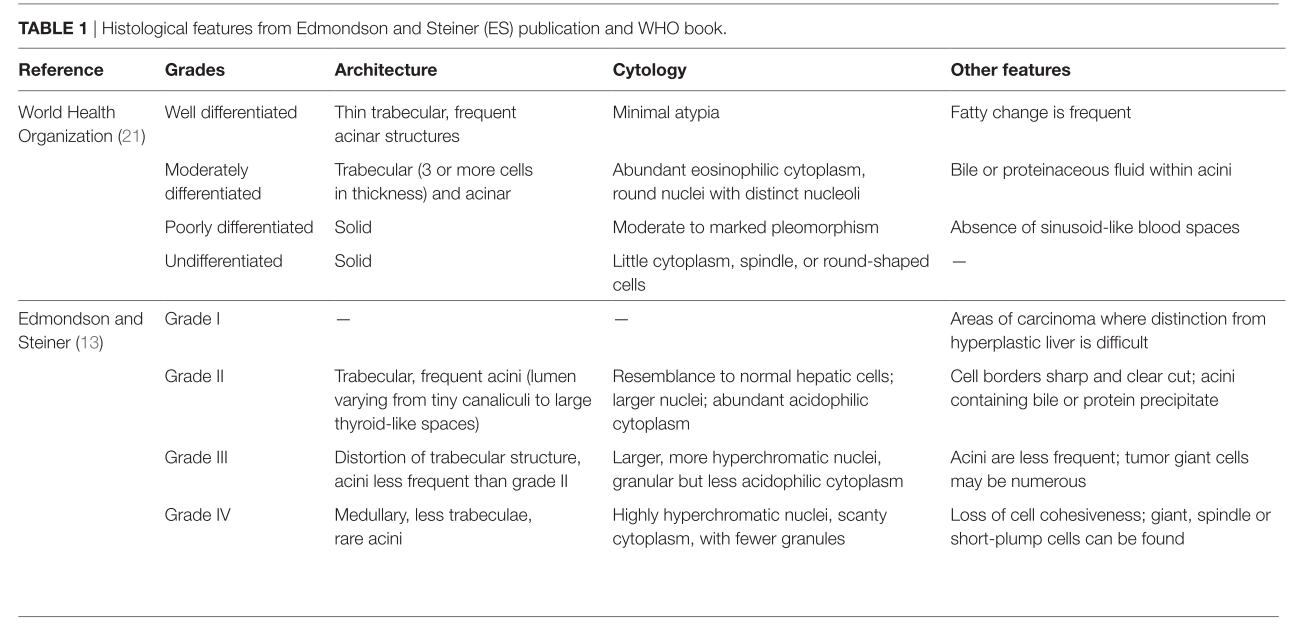
\includegraphics[width=6.26772in,height=3.01389in]{./images/media/image4.png}\\
Even if ES 1954 is the most widely used grading system, a lot of
divergence in the assessment of the grade can be found in the different
studies reviewed by \textbf{Martins et al.}

Some studies suggested that G2 is closer to G1 than to G3 {[}\textbf{ref
15, 16 in Martins et al.}{]}, therefore, a classification that separates
both G1 and G2 in one group and G3 with potentially G4 if available in
the other can be understood.\\
The regroupement of the patients in different numbers of tiers (3 or 4)
G1, G2, G3 and potentially G4, and the possible classification into low
or high differentiation level reveals a high variability in the
assessment of the histological grade, as seen i\textbf{n the following
figure.}

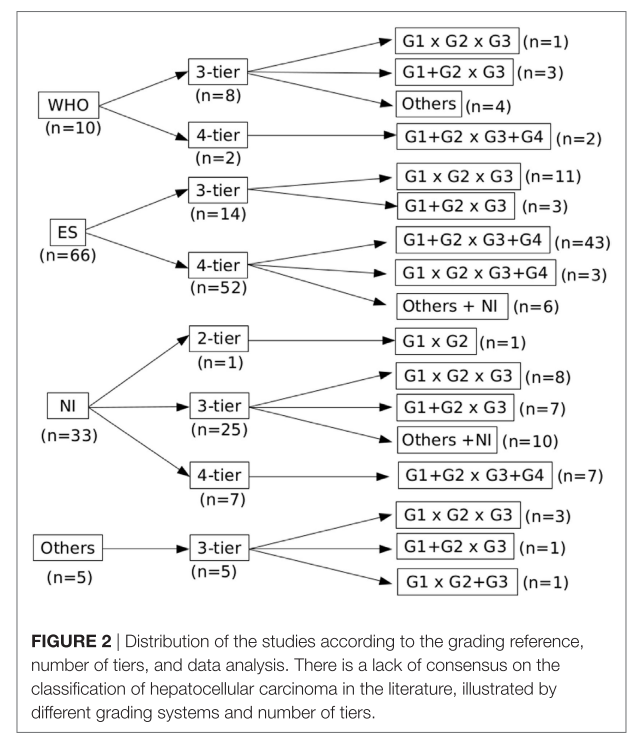
\includegraphics[width=3.49818in,height=4.12223in]{./images/media/image1.png}

\emph{\textbf{Martins et al.}}

This difference in the classification of the patients was also noticed
by \textbf{Han et al, and detailed in the following table.}

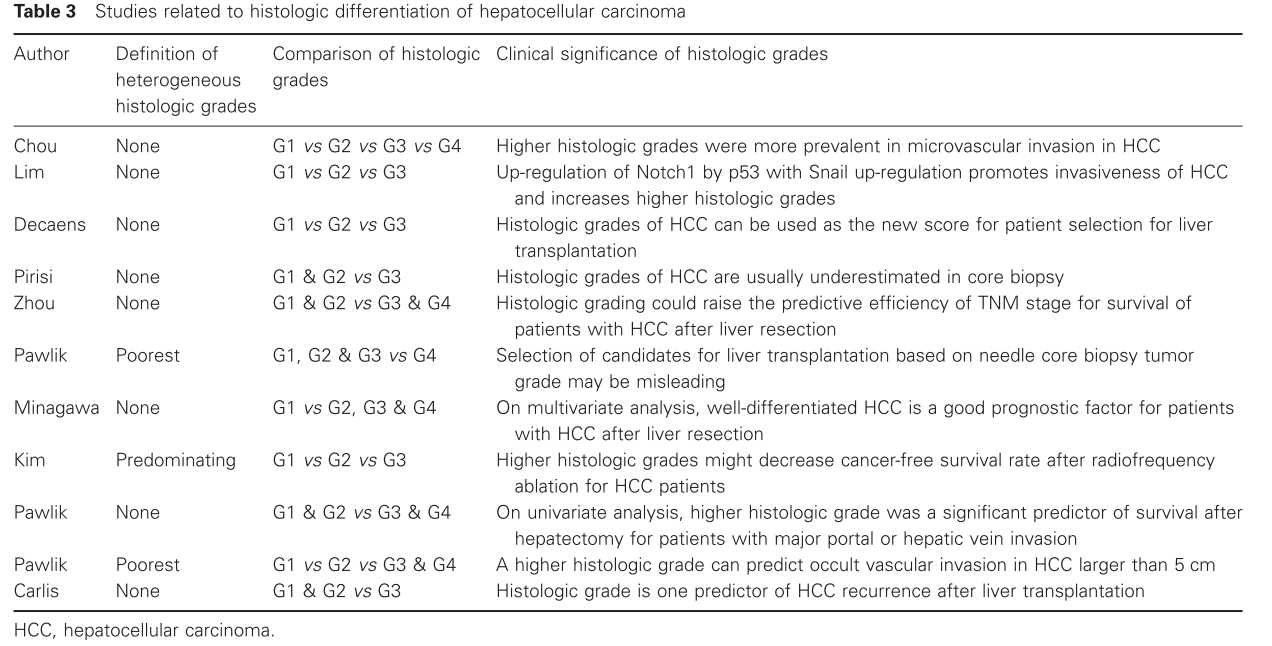
\includegraphics[width=6.26772in,height=3.18056in]{./images/media/image9.png}
They reviewed different articles that used the histological grade to
predict the prognostic of the patients, and realized that no clear
guidelines were given for tumor presenting regions with heterogeneous
grades (\textbf{example of heterogeneous HCC histological slice given
below}).

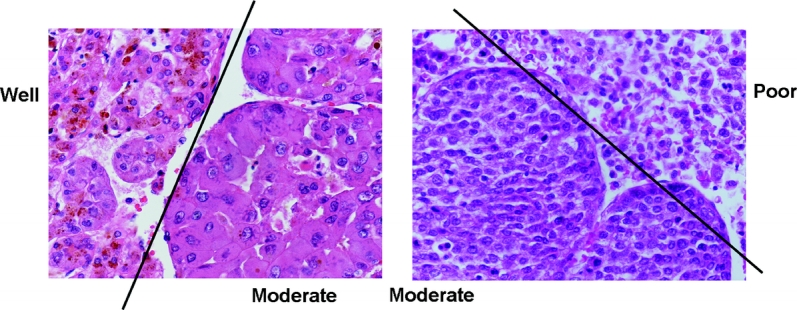
\includegraphics[width=6.26772in,height=2.44444in]{./images/media/image6.jpg}

\emph{Pawlik et al. 2007 © 2007 Lippincott Williams \& Wilkins, Inc.}

The two possible solutions were to consider the worst grade (as
recommended by the ES grading system), or to consider the most present
one (recommended by the WHO grading system), however clear explanations
of the decision taken in such cases are often undisclosed in the
different studies.

The question regarding which histological HCCs grading system to use
remains open. Moreover, various teams proposed to introduce a more
complete grading system where the different features are classified
separately as suggested by \textbf{Martins et al. and depicted in the
following figure}

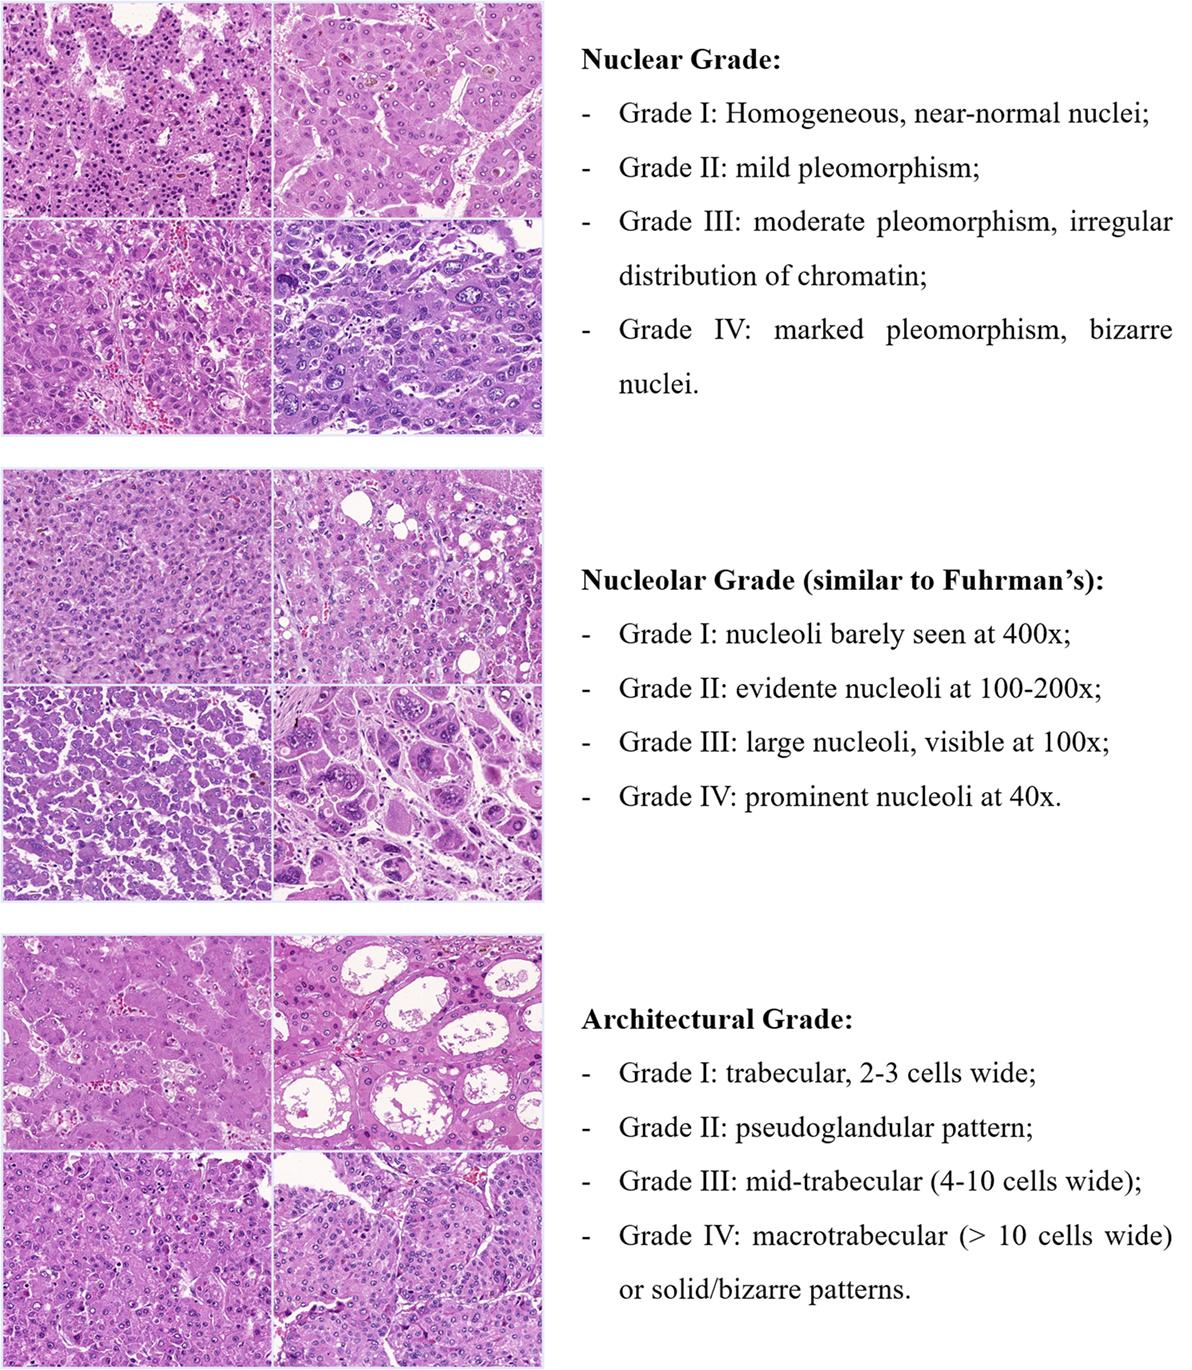
\includegraphics[width=6.26772in,height=7.20833in]{./images/media/image20.jpg}

It is common to differentiate between the \textbf{clinical and the
pathological} grade, where clinical corresponds to the assessment
performed preoperatively, and pathological corresponds to the evaluation
of the sample collected during the surgery.

Some studies even suggested that preoperative histological grades are
not accurate enough to be used as a prognostic factor, and that because
of the high difference between NCB (needle core biopsy) grade and the
one obtained from the final surgical specimen (resulted from the
analysis of samples collected during surgery). \textbf{Pawlik et al.}
exposed the differences between the clinical and the pathological grade
estimation \textbf{in the following table}.

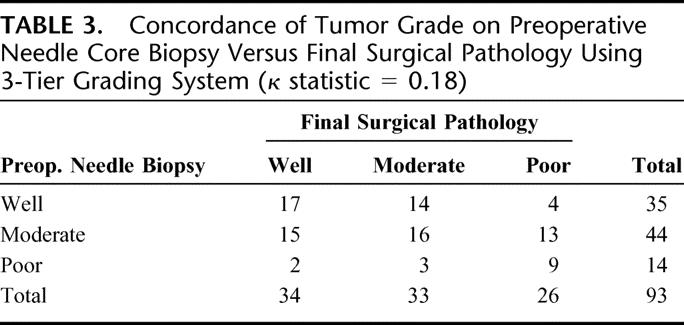
\includegraphics[width=6.26772in,height=2.97222in]{./images/media/image3.jpg}

\emph{Pawlik et al. 2007 © 2007 Lippincott Williams \& Wilkins, Inc.}

As a conclusion, the problem regarding the histological classification
of HCC remains open. Two standards are widely used, namely the ES one
from 1954 and the WHO from 2010. They both initially contain 4 groups,
but differ in the features to consider and the way heterogeneous lesions
are supposed to be classified. When different grades are encountered in
the lesion specimen, ES 1954 recommends to consider the worst one,
whereas WHO 2010 recommends to consider the most frequent one. New
grading systems were introduced lately in order to overcome these
specific problems.

We will now focus on the only study in the literature that tackled the
problem of predicting the histological grade of HCCs through a DL
architecture with medical images, before presenting our own automatic DL
pipeline.

\subsection{DLR based study to predict the histological HCC
grade}\label{dlr-based-study-to-predict-the-histological-hcc-grade}

To our knowledge, only one study tackled the estimation of the
histological grade of HCCs using a DL architecture, but with MR images
as input~{[}\textbf{cite Yang et al. 2019}{]}.

42 patients suffering from HCC were incorporated in their study,
resulting in a total of 51 HCCs. Each lesion was analyzed by 2
experienced pathologists who estimated their histological grade after
microscopic examination (the lesions were classified as well, moderately
and poorly differentiated, following the WHO classification system) .
The extracted tissues were obtained through either biopsy (12 patients)
or after surgical removal (2 liver transplants and 28 liver resection).
All the 42 patients underwent pre-operative multiphasic MR imaging
examinations and images were available at 5 different phases
(Precontrast, late arterial, portal venous, equilibrium and delayed
phases)

They obtained a dataset composed of 9 well, 7 poorly and 35 moderately
differentiated HCCs.

For each patient, a ROI was placed by one expert at the maximal
cross-sectional area to entirely cover the tumor. The same ROI was
copied in the 2 slices above and below the chosen one, to obtain a 3D
volume. Intensities of each volume were normalized and 4D tensors were
created for each patient so that each tensor had a 32x32x5x5 shape
(32x32 corresponding to the resample axial ROI dimension, the third
dimension being the number of retained slices where 2 slices above and
below the chosen one were incorporated, and the last dimension being the
dynamic temporal evolution of the ROI with the 5 phases).

The used architecture \textbf{is depicted below.} It first splits the 4D
tensors into 5 3D objects so that each slice is treated separately. Each
3D volume was then processed by 2 convolutional, 2 max pooling and 1
fully connected layer. The features of each slice were then
concatenated, before a second fully connected layer followed by a dense
layer with a softmax activation function outputs the probability of
belonging to each one of the three classes.

During the training process, they implemented a label-shuffling method
to overcome the problem of imbalance data. Furthermore, to avoid the
effect of overfitting, they trained their network with augmented data
(original images were transposed, rotated, and flipped), a learning rate
reduction and the addition of dropout (rate = 0.5).

Using their architecture they were able to correctly classify the HCCs
into the 3 differentiation groups with a mean accuracy of \textbf{74\%}.

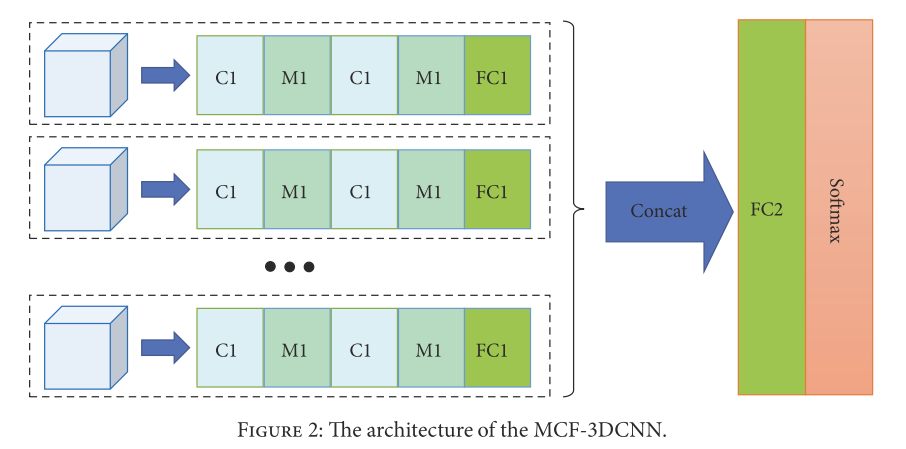
\includegraphics[width=6.26772in,height=3.11111in]{./images/media/image14.png}

Their study however suffers from a lot of limitations such as the
reduced size of the cohort, the imbalance data and the fact that the
analysis was only performed in a manually drawn VOI.

We have decided to tackle the same issue, but we implemented a fully
automatic pipeline where both the segmentation and the grade prediction
steps were performed by DL networks.

\section{Experimental workflow}\label{experimental-workflow}

TCIA-dB is the only open dataset where both tomographic images and
histological grade ground truth are available. It originally only
contained raw images without annotations, so an expert performed the
delineations for both the tumor and the necrosis areas, but both were
done on the PV images only.

In order to perform the prediction of the histological grade, the idea
is to use the imaging features retained for the liver tissue
segmentation, especially those used to segment the tumor and the
necrosis.

We believe that one easy way to extract relevant imaging features is to
use those retained by the semantic segmentation networks, thus the
better the accuracy regarding the semantic segmentation of the liver
tissues, the more accurate the histological grade prediction will be.

As explained previously, we proved that a cascaded architecture combined
with the use of temporal contrast enhanced images allows a better
delineation of liver tissues. Using temporal information can potentially
improve the accuracy of the grade prediction, by exploiting the wash-in
wash-out specific features {[}\textbf{cite Okamoto2012}{]}.

To conduct our DLR study, we chose first to perform a multiphasic
semantic segmentation of the TCIA-dB, before trying to predict the
histological grade.

\subsection{Registration}\label{registration}

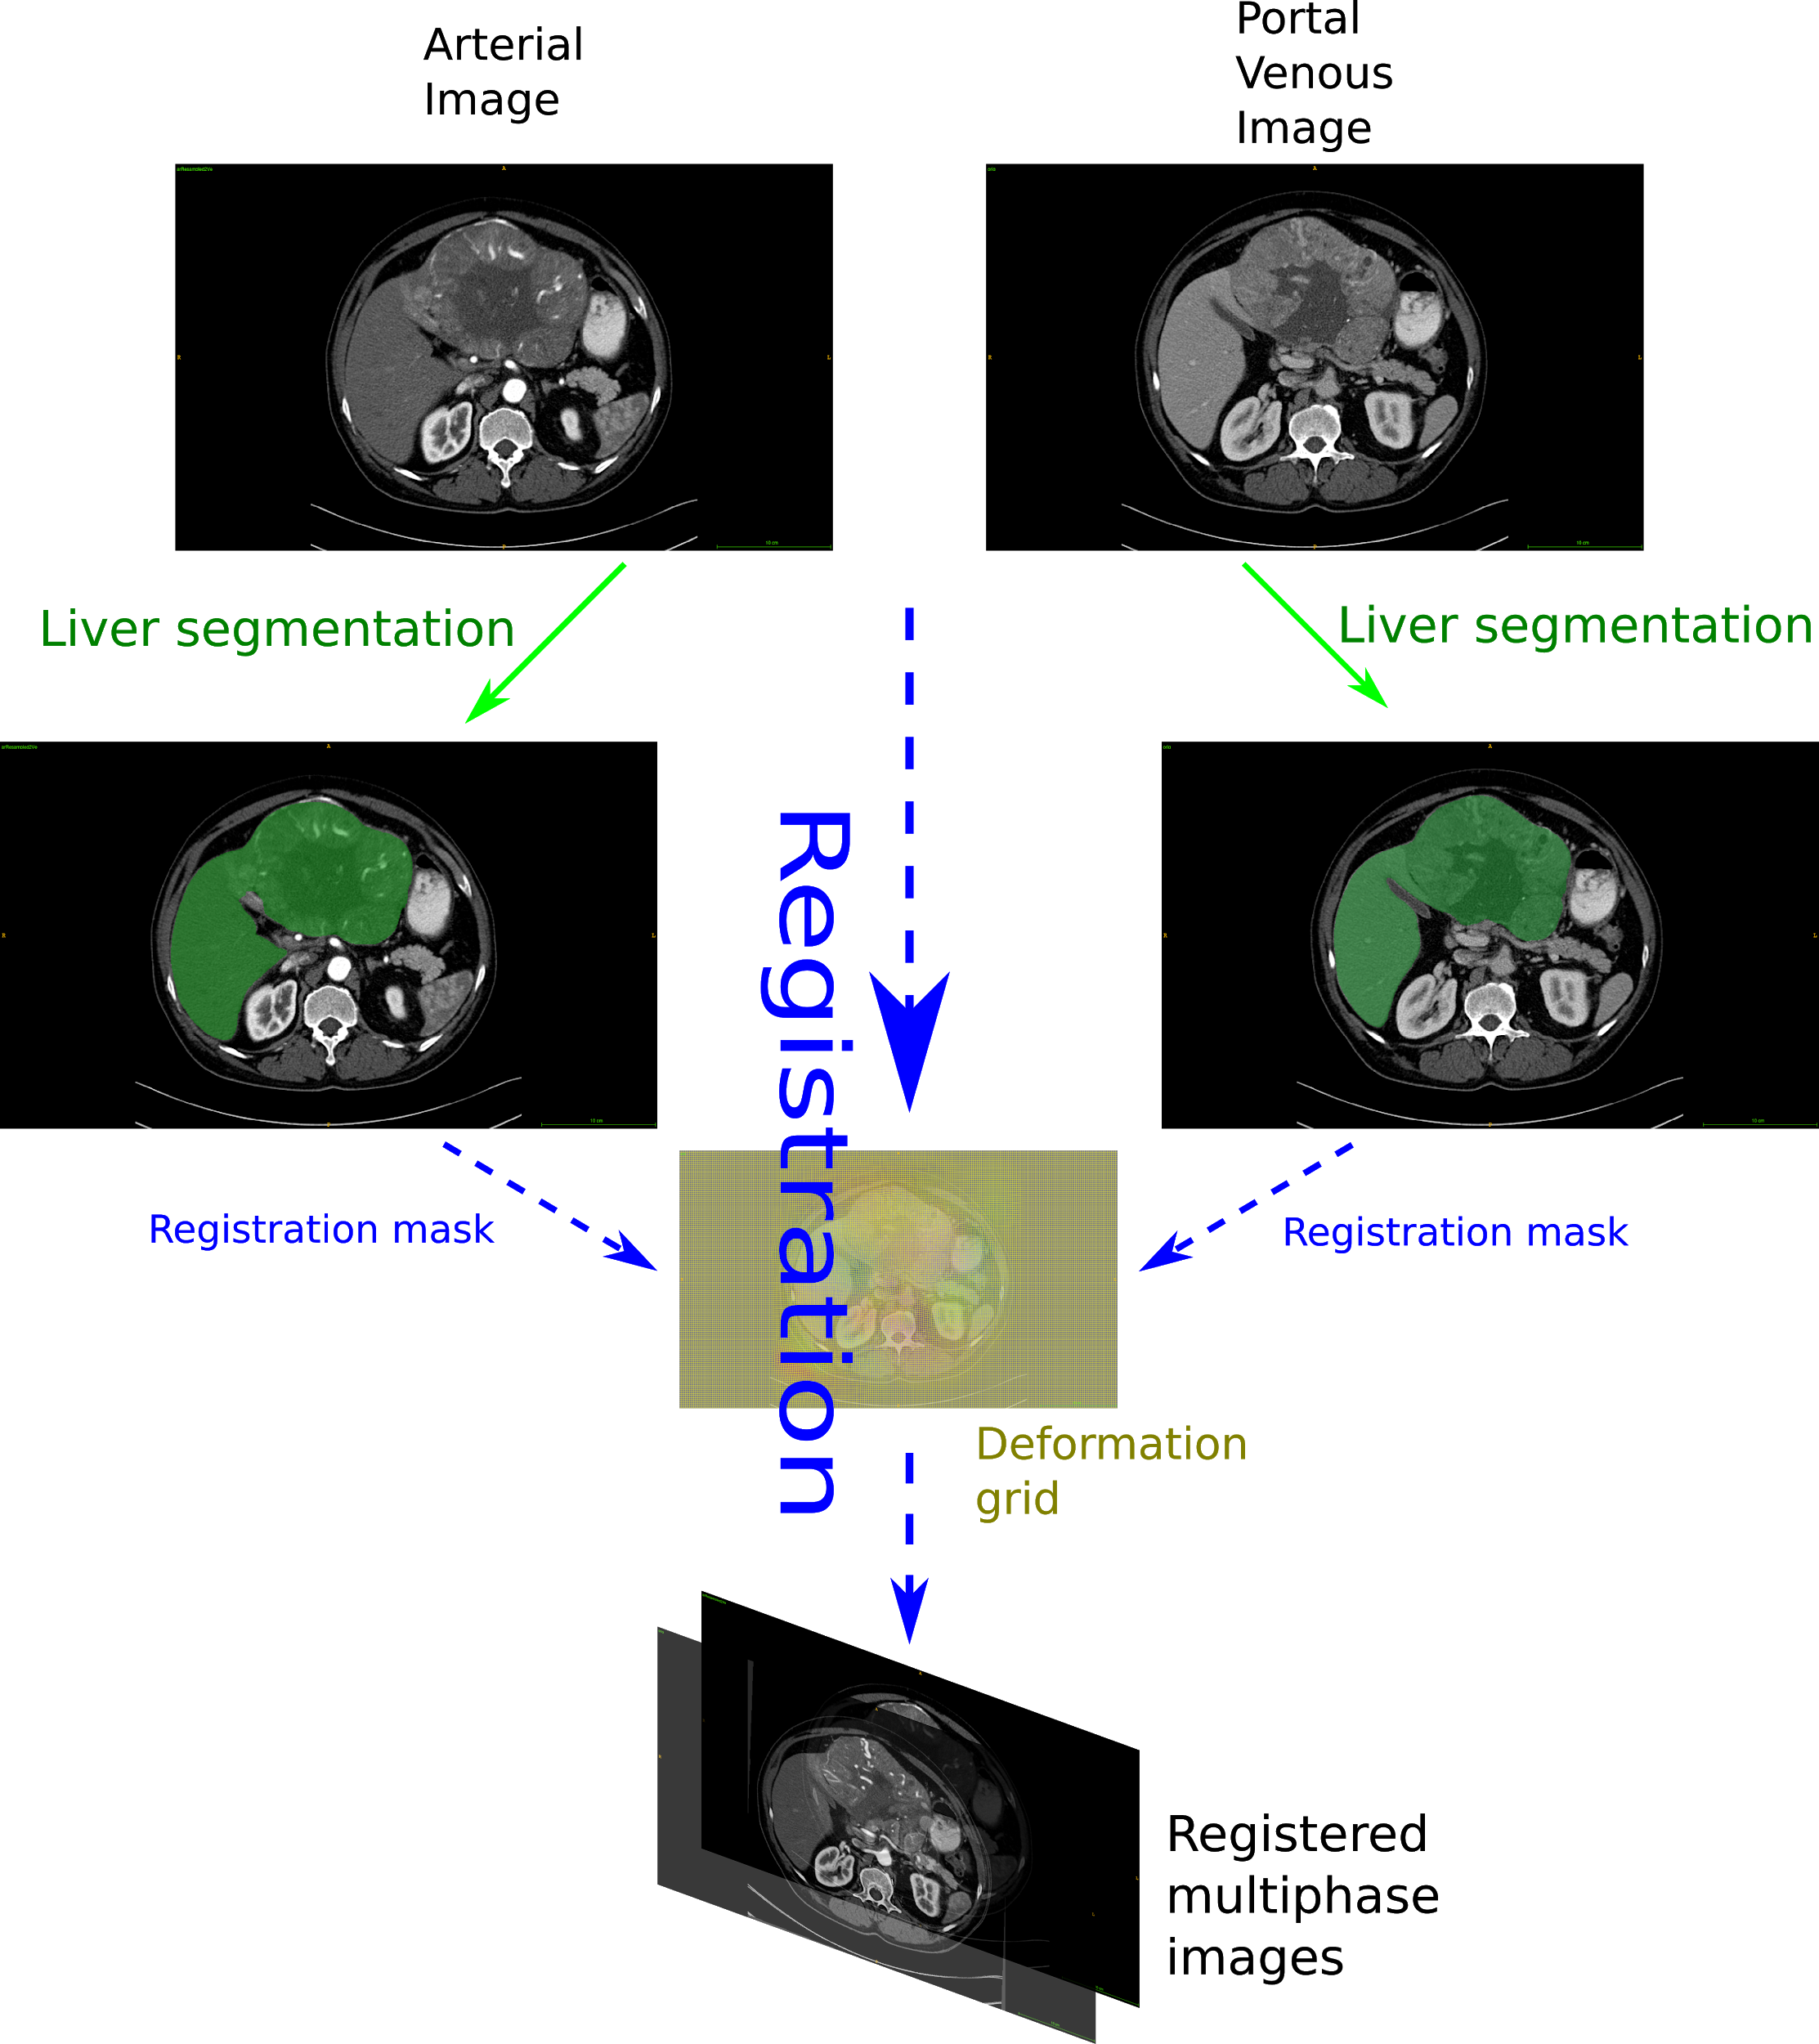
\includegraphics[width=6.26772in,height=7.04167in]{./images/media/image24.png}

\emph{Illustration of the registration pipeline applied to the images of
the TCIA-dB. The first green arrows correspond to the liver segmentation
using a network trained on the LITS-dB. Dashed blue arrows correspond to
the ANTs registration pipeline, where a dilated version of the predicted
liver annotations maps are used as registration masks. The ANTs
algorithm implements 3 transformations: a rigid, an affine, and
diffeomorphic Syn transformation that computes a deformation grid
{[}}\href{https://sci-hub.do/10.1016/j.media.2007.06.004}{\emph{\emph{Avants2008}}}\emph{{]}.
The 3 steps of the ANTs call allows us to obtain registered multiphase
images.}

To achieve a multiphasic semantic segmentation of the liver tissues we
have to ensure that both the liver and its internal structures such as
the potential tumors are located at the same spatial position between
the different CECT volumes.

One way to perform a registration is to implement a series of
transformations (rigid or non-rigid) that will match a moving volume to
a target one. Each step of the registration is controlled by a
similarity loss.

When dealing with CT volumes the available losses controlling the
different steps of the registration pipeline can be affected by areas of
the body with a high gradient such as the bones for example. When
registering two CT volumes, one can either directly use both the entire
volumes or constraints the registration to a specific area (aka mask).

The liver being a soft organ, it easily moves with the respiratory
motions, in order to reduce the effect of the neighboring parts of the
abdomen, we have decided to restrict the computation of the symmetric
metrics to the dilated liver mask area so that the registration
algorithm mainly focus on the gradient present along its borders.

Therefore, the first step for the TCIA-dB registration is to perform a
liver semantic segmentation (\textbf{green arrows in the registration
pipeline figure}).

\subsection{TCIA-dB unsupervised liver
segmentation}\label{tcia-db-unsupervised-liver-segmentation}

In the available datasets (\textbf{ref table}), only TheraHCC-dB and
LITS-dB contained liver expert's delineation.

TheraHCC-dB contains annotations only on sparse slices across the liver,
whereas LITS-dB contains full 3D pixel-wise liver annotation but it only
contains monophase images, without any information regarding the
acquisition phase.

Our experiments however showed that a liver segmentation network trained
on sufficiently enough cases is able to perform the semantic
segmentation of both AR and PV raw images independently.

We trained our network called CECT-Liver on the 131 volumes of the
LITS-dB following using the same hyperparameters as the ones detailed
previously. When testing the CECT-Liver network on TheraHCC-dB we
obtained a mean slice-wise DSC of 90.4 +/- 17.5 on the PV images and
86.9 +/- 19.1 on the AR images. Those results, close to those obtained
in our previous work using a CV approach, proved that CECT-Liver can
perform liver segmentation on both AR and PV unseen images.

The CECT-Liver network was also able to segment unseen volumes of the
TCIA-dB in both AR and PV phases even when the liver presents a big
lesion, as we can see \textbf{in the images below}.

\begin{longtable}[c]{@{}ll@{}}
\toprule
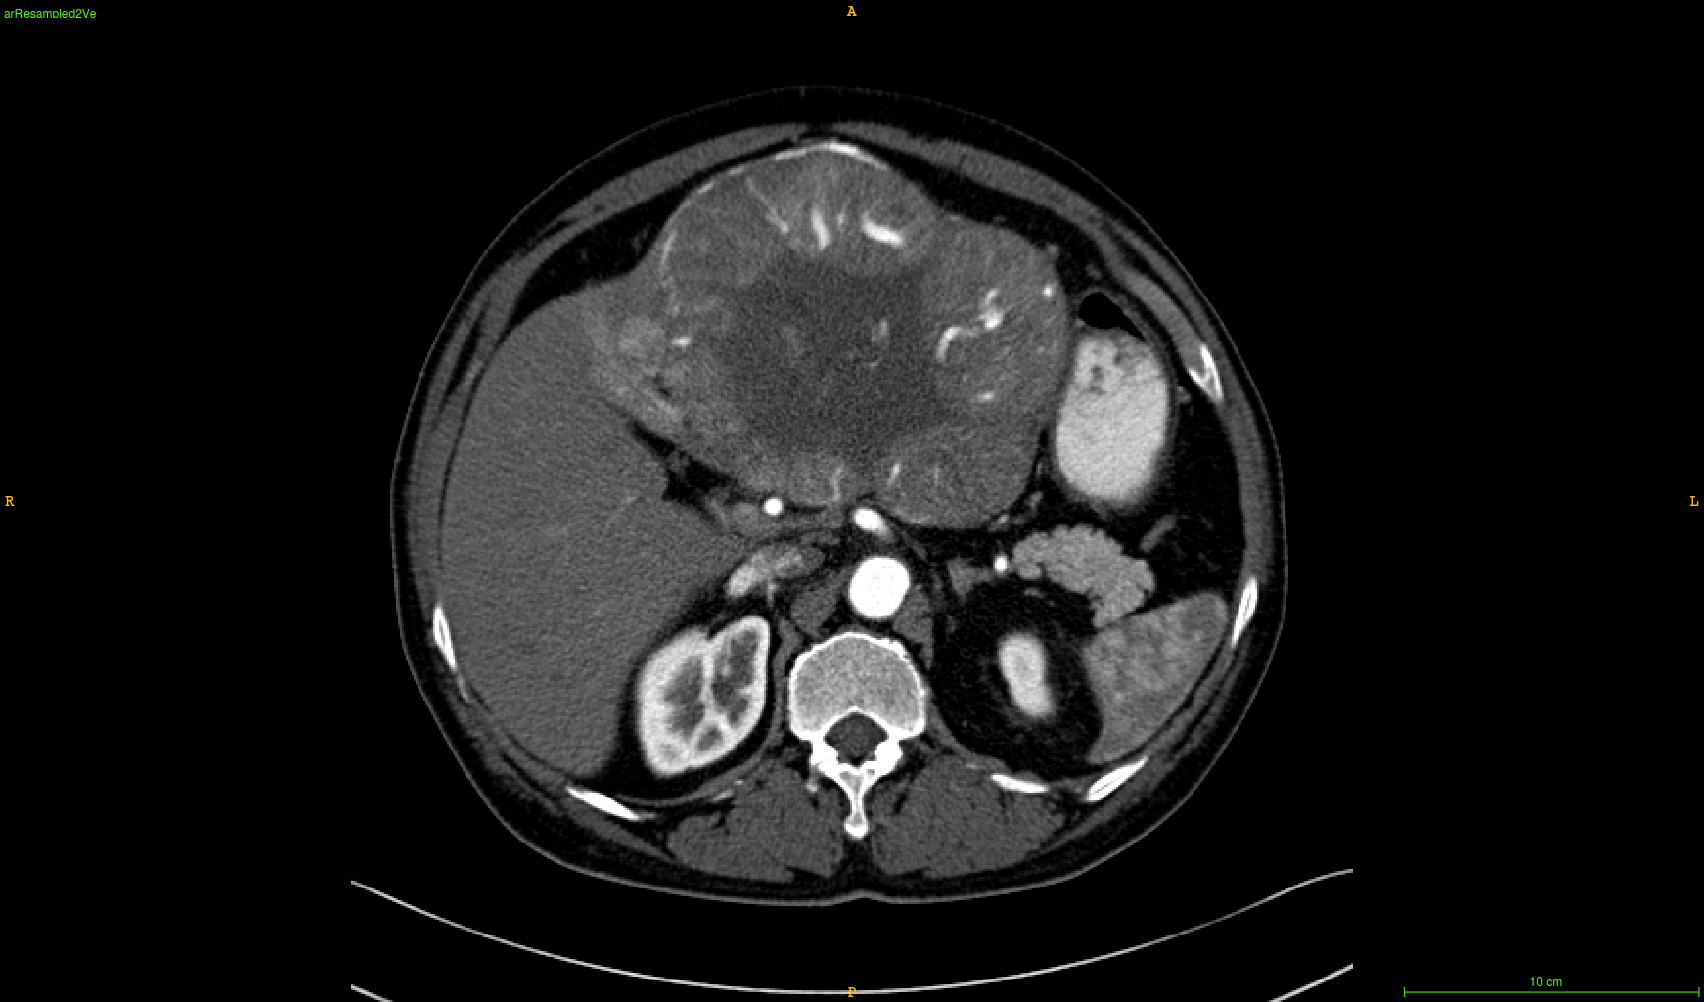
\includegraphics[width=2.97917in,height=1.75000in]{./images/media/image11.png}
&
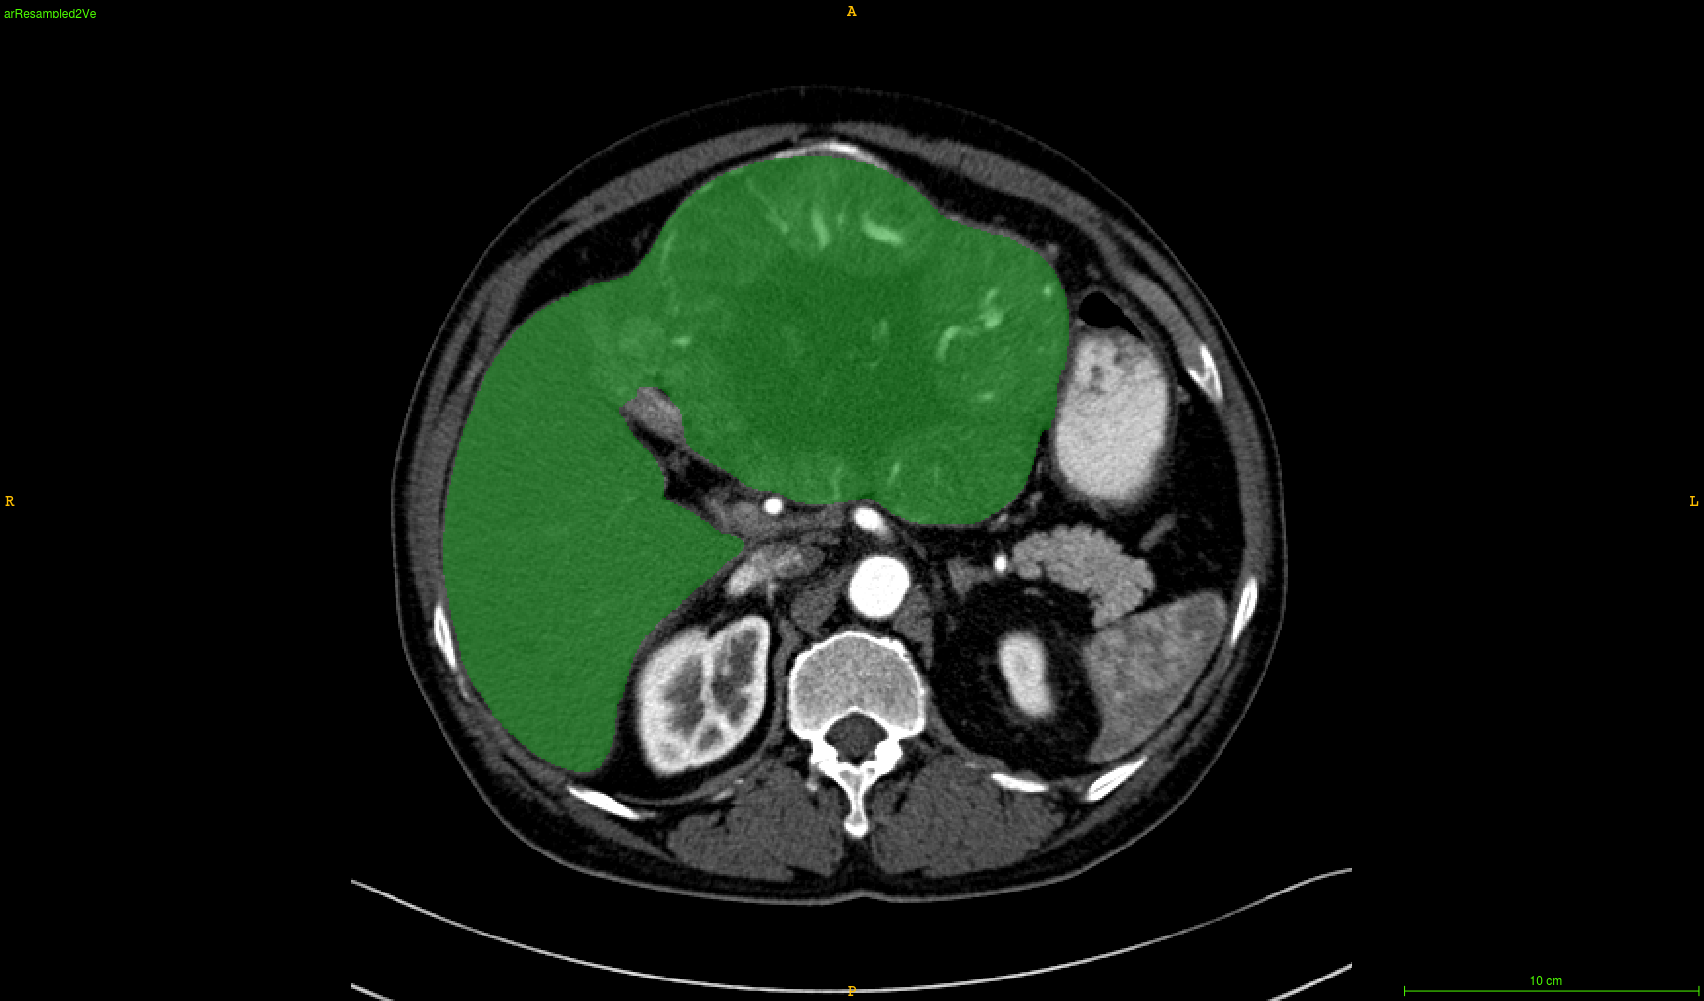
\includegraphics[width=2.97917in,height=1.75000in]{./images/media/image12.png}\tabularnewline
\midrule
\endhead
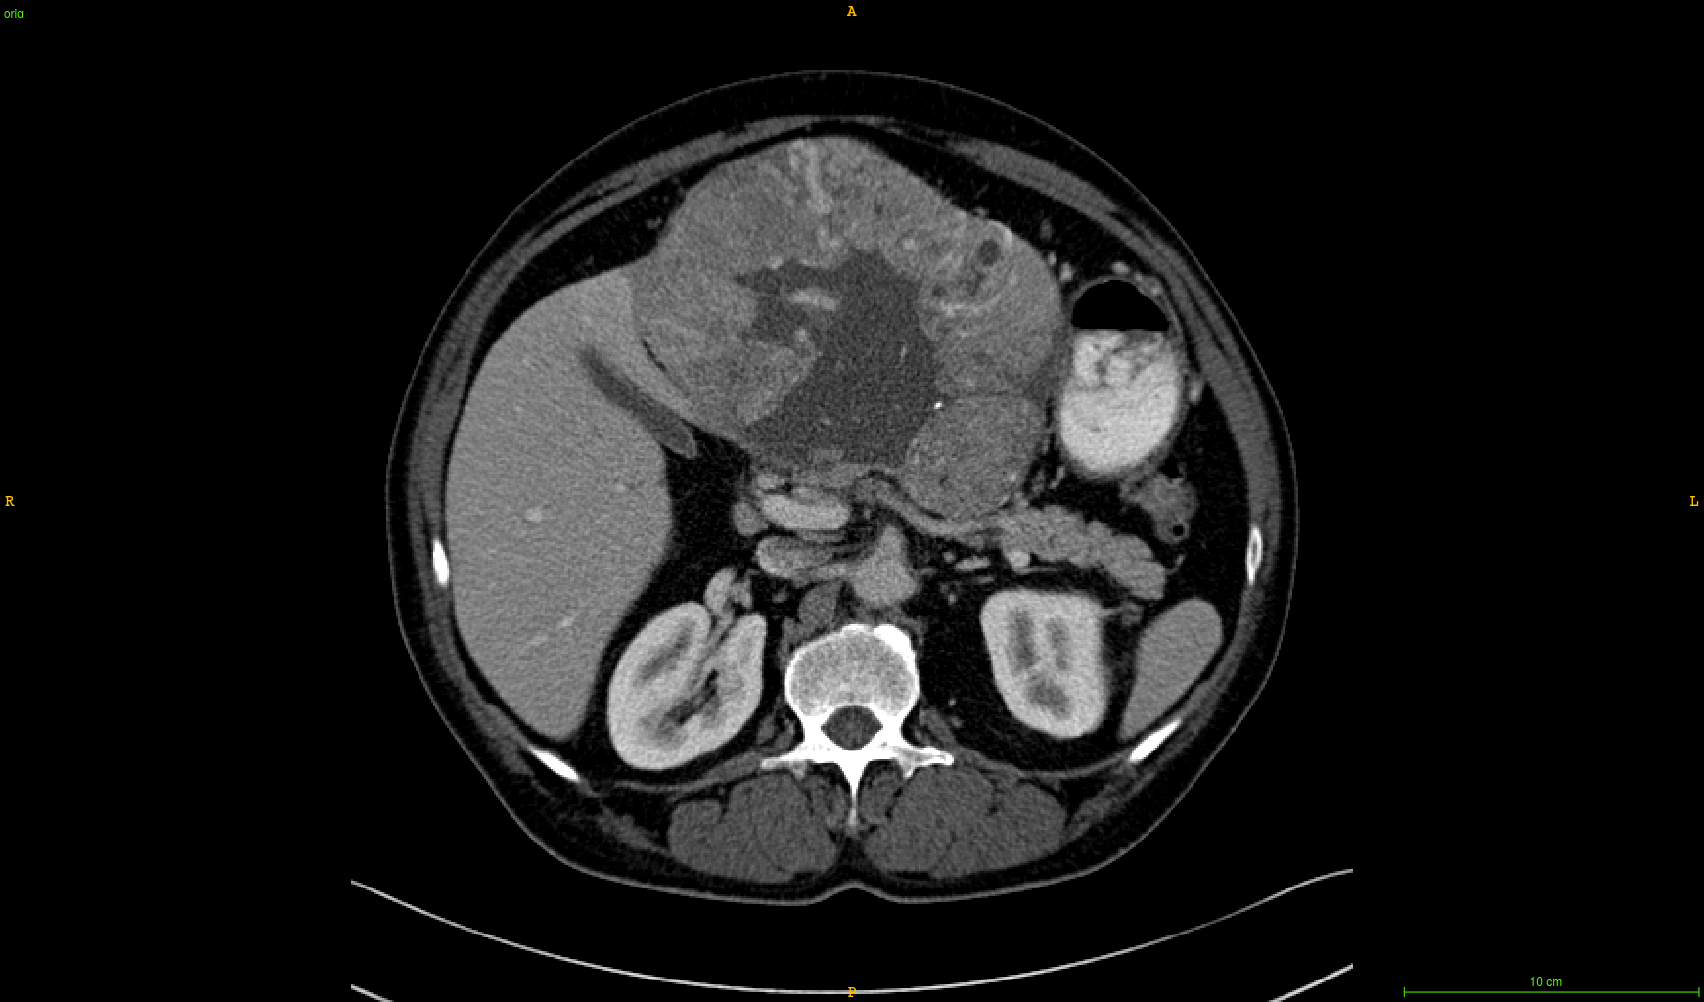
\includegraphics[width=2.97917in,height=1.75000in]{./images/media/image16.png}
&
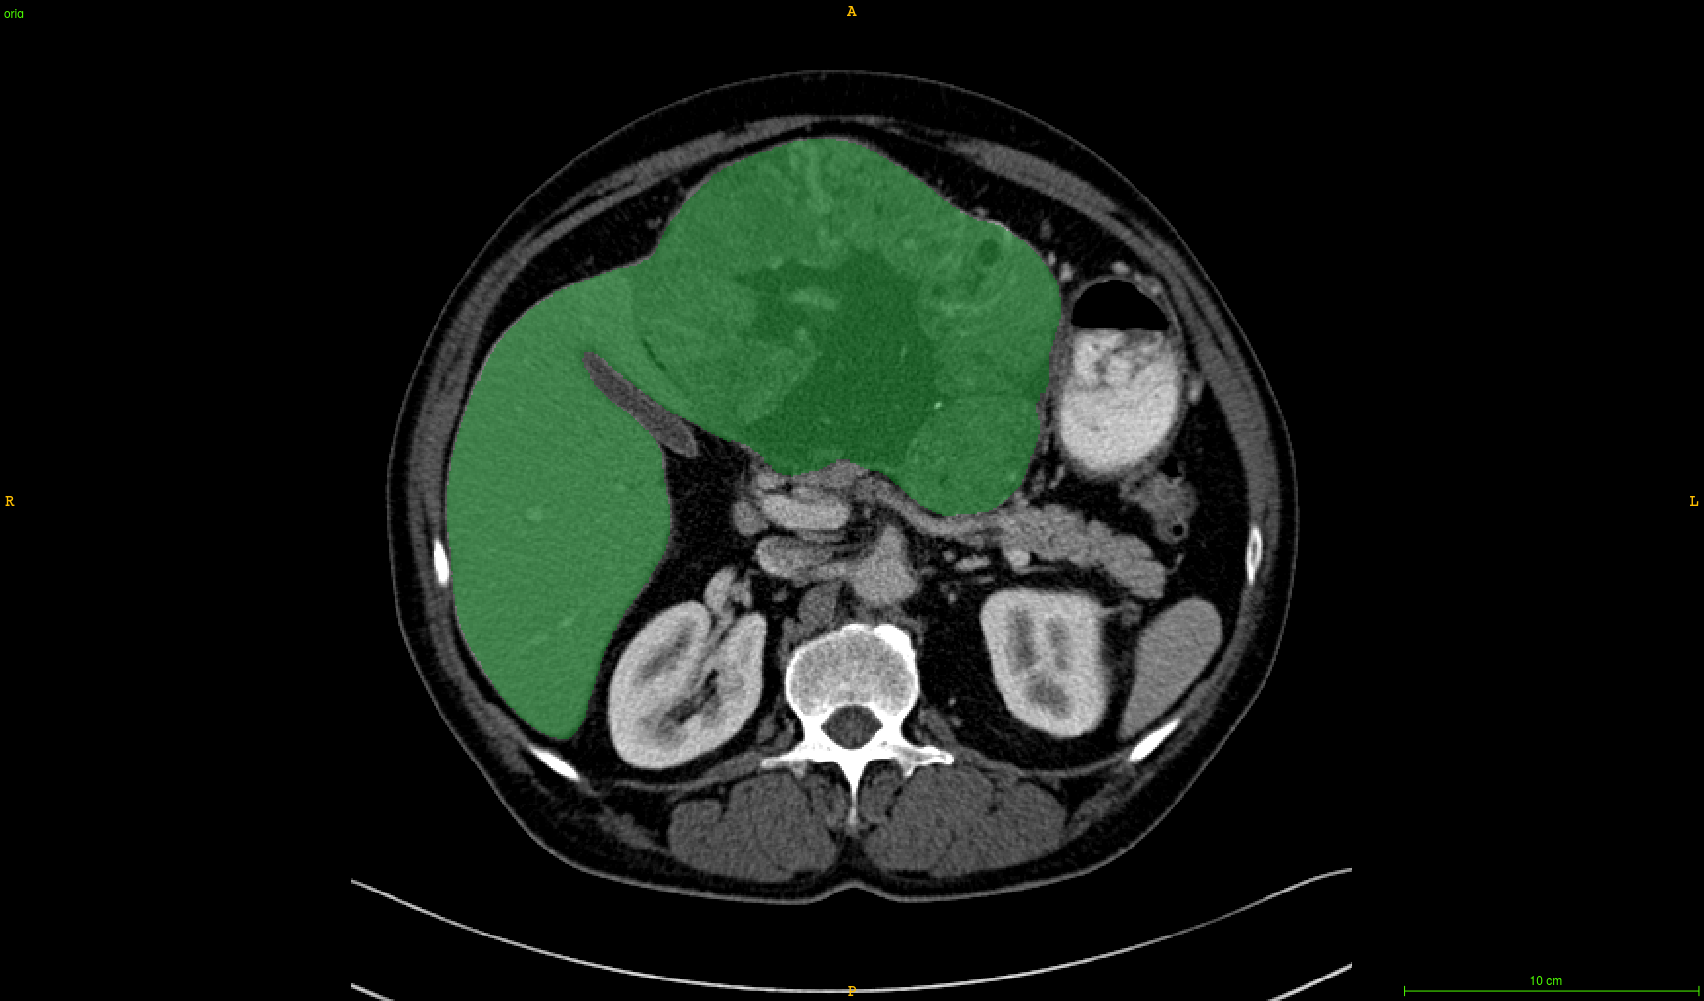
\includegraphics[width=2.97917in,height=1.75000in]{./images/media/image18.png}\tabularnewline
\bottomrule
\end{longtable}

Example of liver segmentation using the CECT-Liver network on TCIA-dB
patients (Top row AR phased images, bottom row: PV phased images, left:
Raw images, right : liver segmentation as overlay).

Once a robust liver segmentation was obtained, we implemented our
registration pipeline.

We have decided to implement the registration pipeline using ANTs
(\textbf{cite ANTS mendeley}), since it has been already used for liver
CT scans registration {[}cite
\href{https://openaccess.thecvf.com/content_ICCV_2019/papers/Zhao_Recursive_Cascaded_Networks_for_Unsupervised_Medical_Image_Registration_ICCV_2019_paper.pdf}{\emph{Zhao
2019}}, \href{https://arxiv.org/pdf/1902.05020.pdf}{\emph{Zhao
2019-2}}{]}.

\subsection{TCIA-dB ANTs registration}\label{tcia-db-ants-registration}

The classical ANTs registration pipeline is made of 3 steps. The first
two steps consist of linear transformations, where a rigid
transformation is first applied, followed by an affine transformation.
The last one is generally a non-linear transformation. In our pipeline,
we used a Syn (\emph{Standard Symmetric normalisation}) transform, which
processes a gradient field, determining how each point of the space will
shift {[}cite
\href{https://sci-hub.do/10.1016/j.media.2007.06.004}{\emph{Avants2008}}{]}.

The MI (Mutual Information) was used as loss function for the first two
steps because it has the advantage of computing the similarity at a
large scale. Linear transformations tend to roughly bring both volumes
in the same space so we decided not to use a finer metric. For the Syn
transform, we used the CC (Cross Correlation) as loss function. The CC
has the advantage of looking precisely in a region around each voxel
when computing the similarity between the two volumes.

During the registration process, the liver segmentation was used as
registration mask, and we decided to set the PV volume as target (fixed)
volume since it usually presents the finer voxel resolution when
compared to AR (or DELAY) volume, and since it contains the original
expert annotations.

Registration pipeline:

For a given patient in the TCIA-dB here are the implemented registration
steps:

\begin{enumerate}
\def\labelenumi{\arabic{enumi}.}
\item
  \begin{quote}
  We initially resampled the AR volume so it has the same resolution as
  the corresponding PV volume.
  \end{quote}
\item
  \begin{quote}
  We performed the liver segmentation using CECT-Liver on both the PV
  and the AR\_resampled volumes in a slice\_wise manner with a classical
  post-processing consisting in applying a binary opening operation to
  the mask and conserving the big connected component (\textbf{see green
  arrows in the registration pipeline figure}). We obtained both
  PV\_liver\_mask and AR\_resampled\_liver\_mask volumes.
  \end{quote}
\item
  \begin{quote}
  We applied the registration using both dilated PV\_liver\_mask and
  AR\_resampled\_liver\_mask as registration masks \textbf{as depicted
  by the dashed blue arrows in the registration pipeline figure} (we
  used a dilated version of the liver mask with a SSE of 5cm when
  setting the registration mask in order to counter any error in the
  segmentation process, and to always have both the liver and its border
  included in the registration mask)
  \end{quote}
\item
  \begin{quote}
  The registration allows us to obtain both a new registered arterial
  volume, a transformation matrix and a deformation field volume.\\
  In the axial plane, the obtained deformation fields tend to present
  high deformation at both the top and the bottom of the liver (which
  can be explained anatomically since they are surrounded by the air and
  will be more subject to deformation than central areas of the liver)
  whereas central areas of the liver present high deformation close to
  the border.
  \end{quote}
\end{enumerate}

\begin{longtable}[c]{@{}l@{}}
\toprule
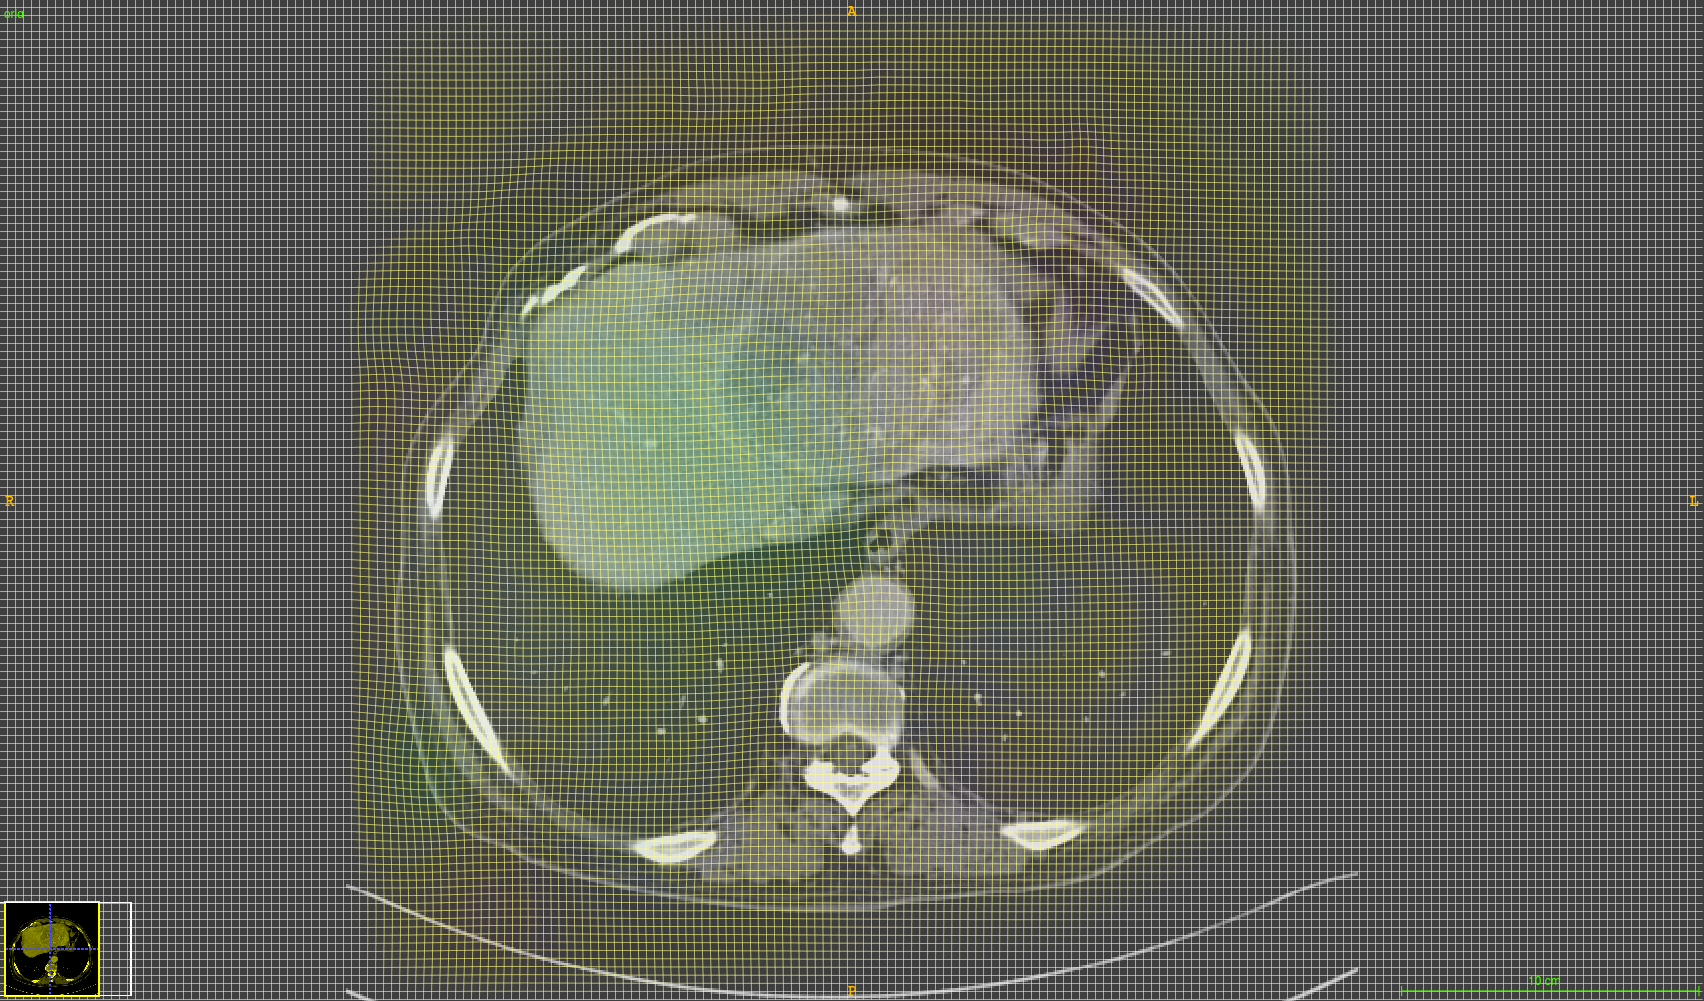
\includegraphics[width=5.61458in,height=3.29167in]{./images/media/image15.png}\tabularnewline
\midrule
\endhead
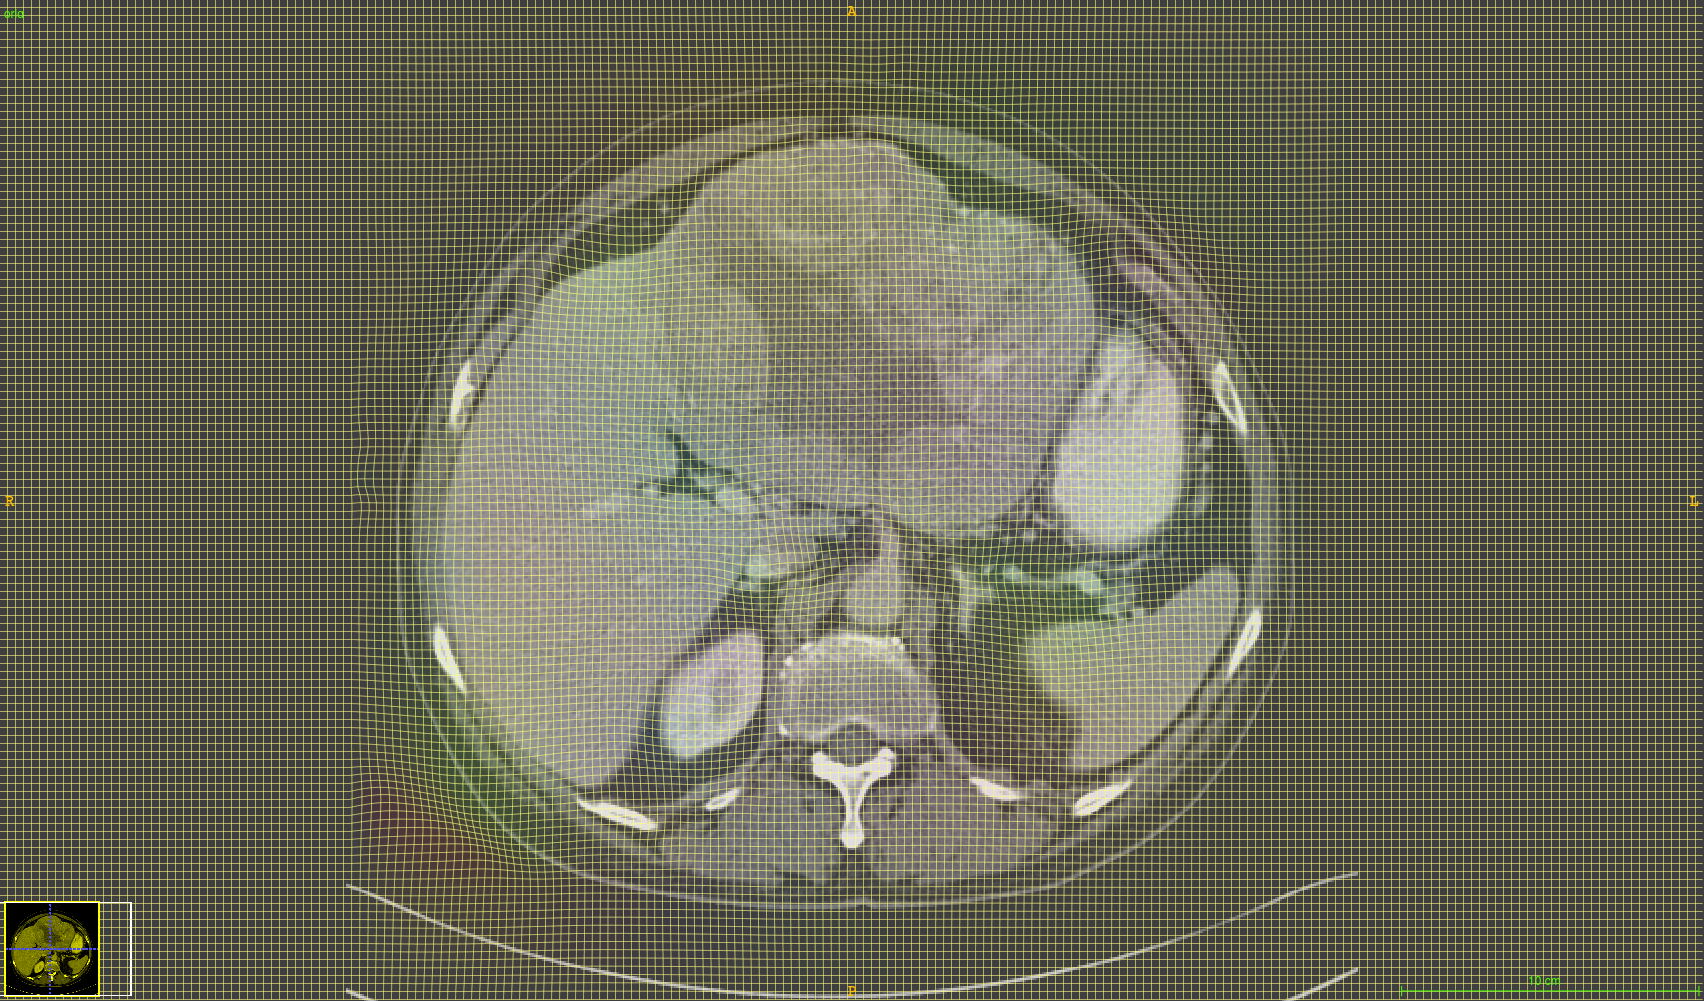
\includegraphics[width=5.61458in,height=3.29167in]{./images/media/image17.png}\tabularnewline
\bottomrule
\end{longtable}

One way to assess the precision of the registration is to apply the
transformation matrix to the initial AR\_resampled\_liver\_mask and to
compute the DSC with the target PV\_liver\_mask. When applying this
evaluation, we obtained a mean patient\_wise DSC of 92.8 +/- 3.8 at the
end of the registration step on the TCIA-dB, sufficient to consider the
registration as successful when compared to state-of-the-art
registration methods
{[}\href{https://openaccess.thecvf.com/content_ICCV_2019/papers/Zhao_Recursive_Cascaded_Networks_for_Unsupervised_Medical_Image_Registration_ICCV_2019_paper.pdf}{\emph{Zhao
2019}}{]}

\subsection{TCIA-dB unsupervised multiphase tumor
segmentation}\label{tcia-db-unsupervised-multiphase-tumor-segmentation}

Once both the AR and PV volumes of the TCIA-dB were registered, and the
liver masks obtained, we built the second step of our cascaded
architecture, dedicated to the multiphasic tumor segmentation. In order
to train such a network, we created a multiphase (arterial and portal
venous) database where the temporal volumes of a given patient are
registered and where segmentations of both the liver and tumor regions
are available.

TheraHCC-dB and G-dB were the only two datasets containing multiphasic
images (as we can see in the \emph{\textbf{dataset table}}), however
G-dB initially contained ground truth annotation only for the tumors,
with segmentations performed only on the AR phase images.

Since G-dB contains more cases than TheraHCC-dB, we have decided to
build our multiphasic tumor segmentation network on this dataset.
However in order to train a tumor segmentation network, our cascaded
architecture requires to have the liver segmentation mask as input for
the second step (as depicted in this figure {[}\textbf{ref figure
Cascade CARS}{]}), therefore we had to obtain the liver segmentation
mask for the patients of the G-dB.

AR and PV volumes of the G-dB dataset were initially not registered so
we applied the same registration pipeline as the one used for TCIA-dB
{[}\textbf{ref registration pipeline}{]}. After applied the procedure to
each patient of G-dB,~we used the resulting transformation matrix to
transform the AR tumor mask to the PV space \textbf{as depicted in the
following figure.}

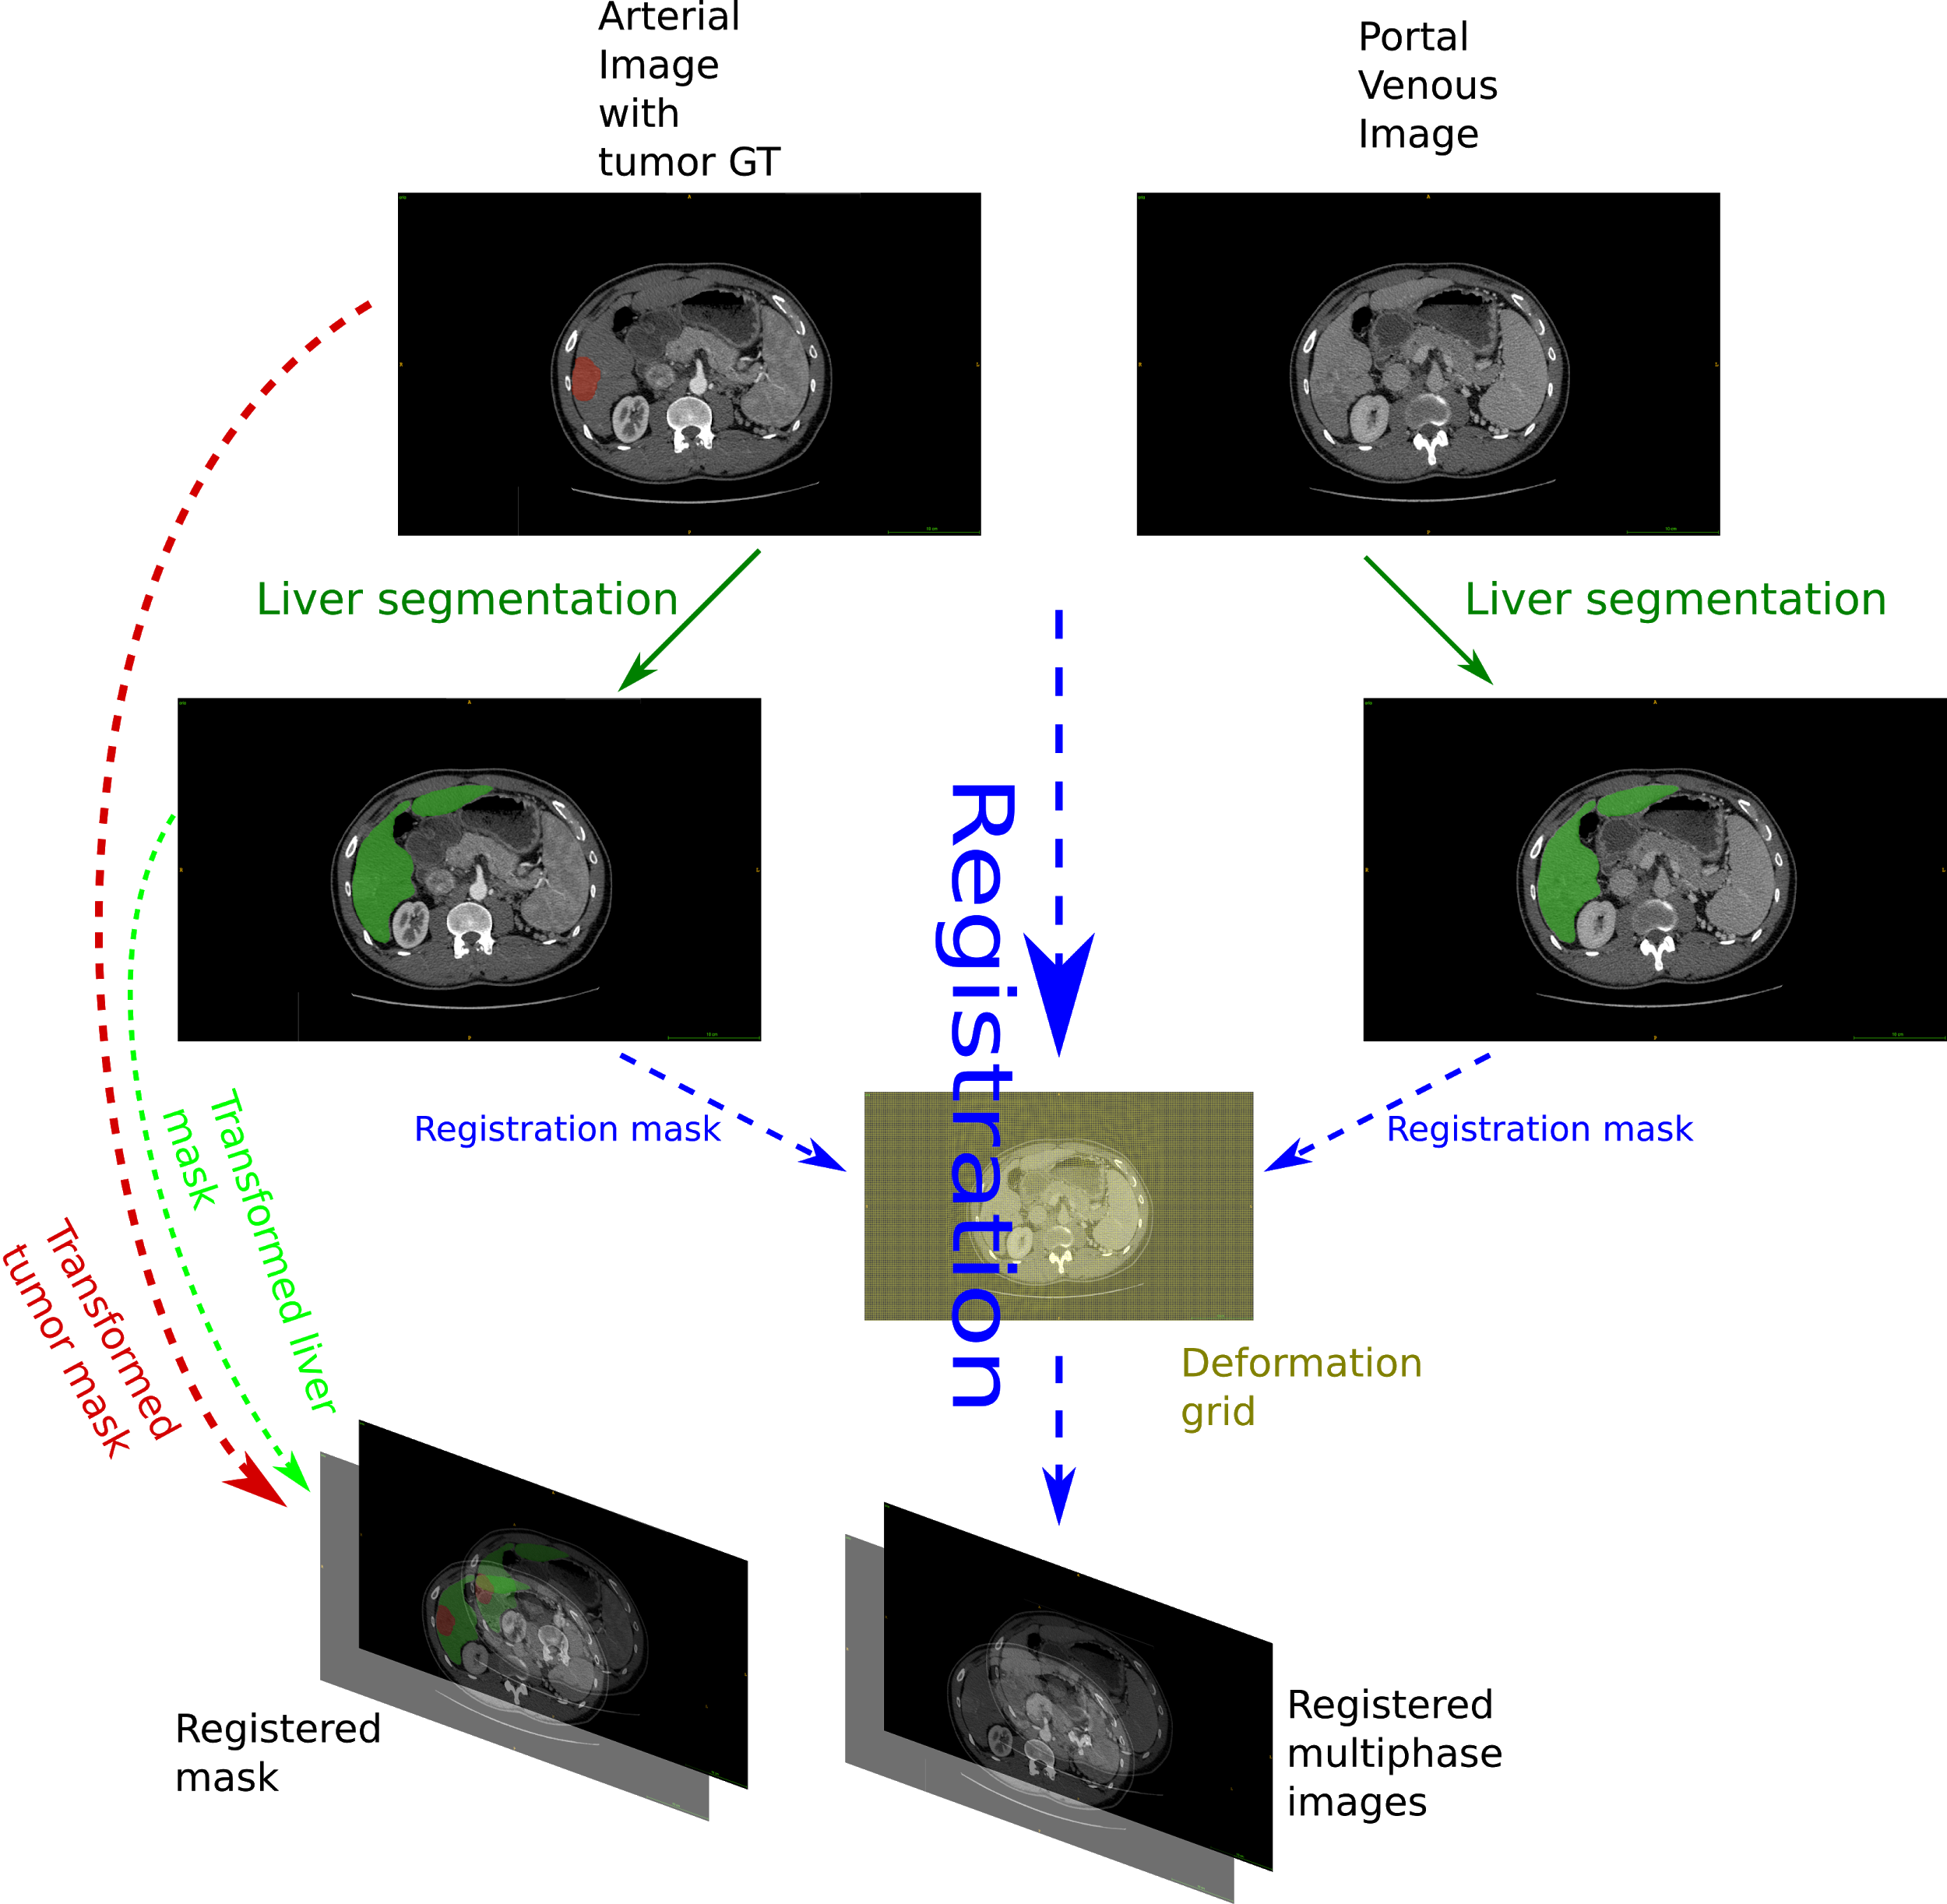
\includegraphics[width=6.26772in,height=6.12500in]{./images/media/image23.png}

\emph{Illustration of the registration pipeline applied to G-dB. A
similar approach as the one applied to TCIA-dB is performed to obtain
the registered multiphase images. A final step is added here to
transform both the tumor and the liver masks using the registration
transformation matrix (red and green dashed arrows).}

We then fused the liver and the tumor mask to obtain a multiclass
segmentation mask that can fit both PV and the AR\_registered volumes,
\textbf{as depicted hereafter.}

\begin{longtable}[c]{@{}ll@{}}
\toprule
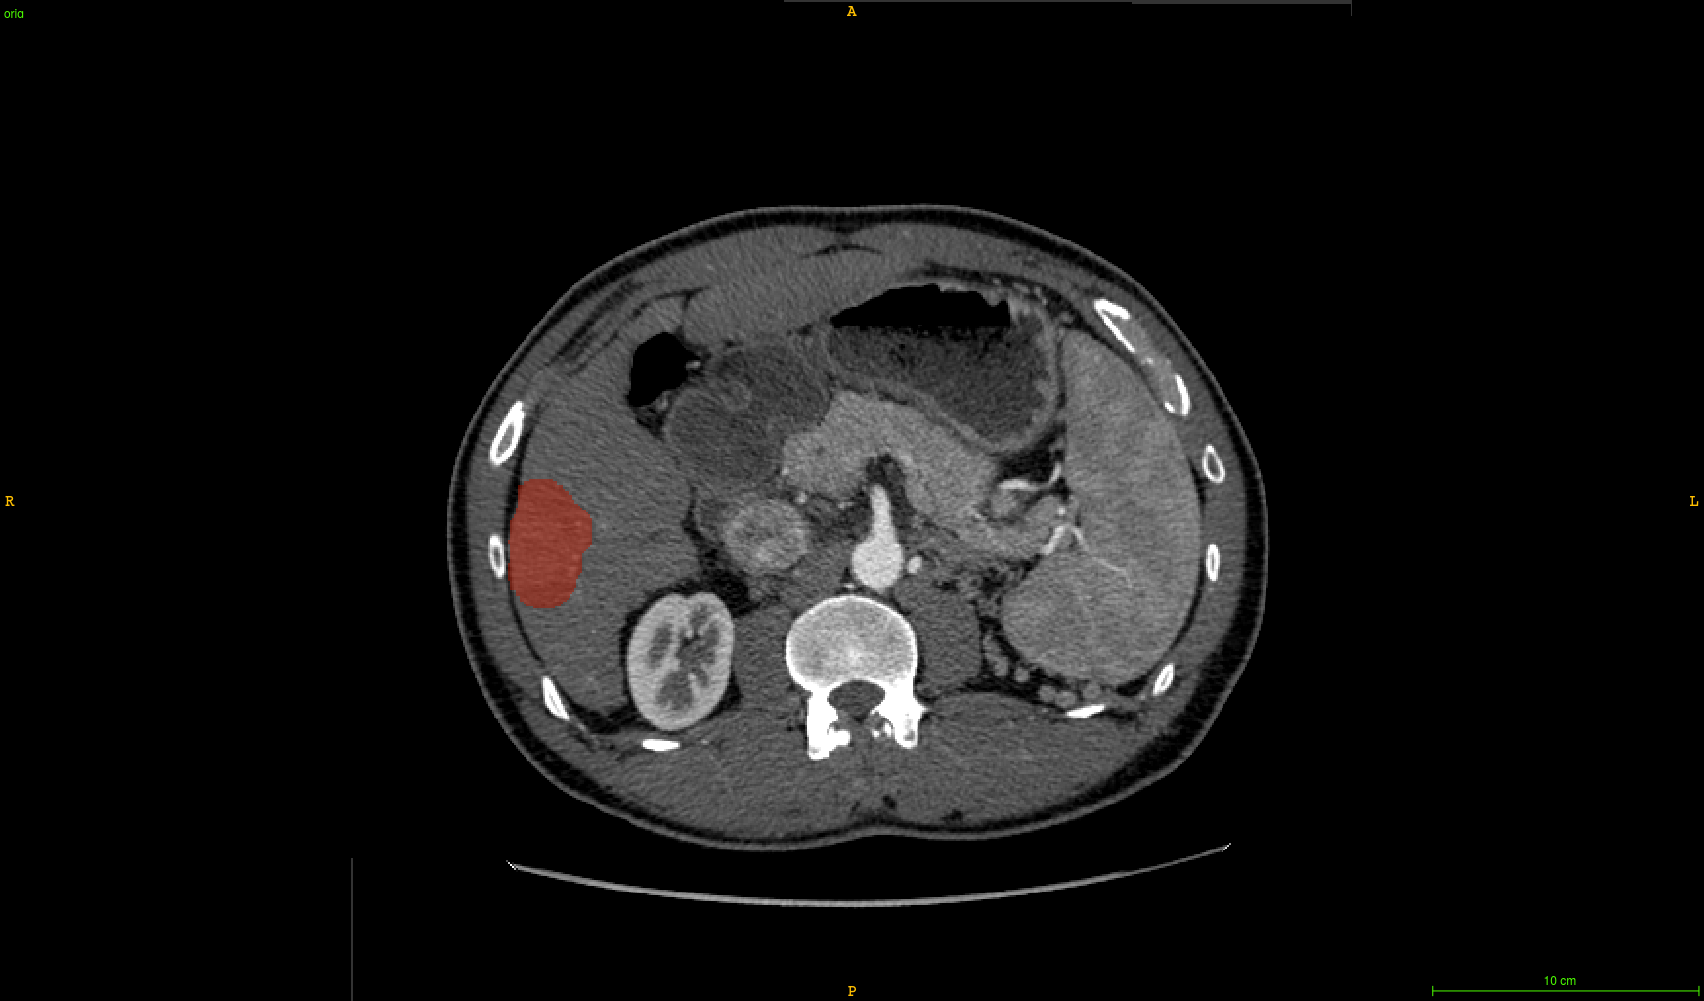
\includegraphics[width=3.10417in,height=3.09722in]{./images/media/image2.png}
&
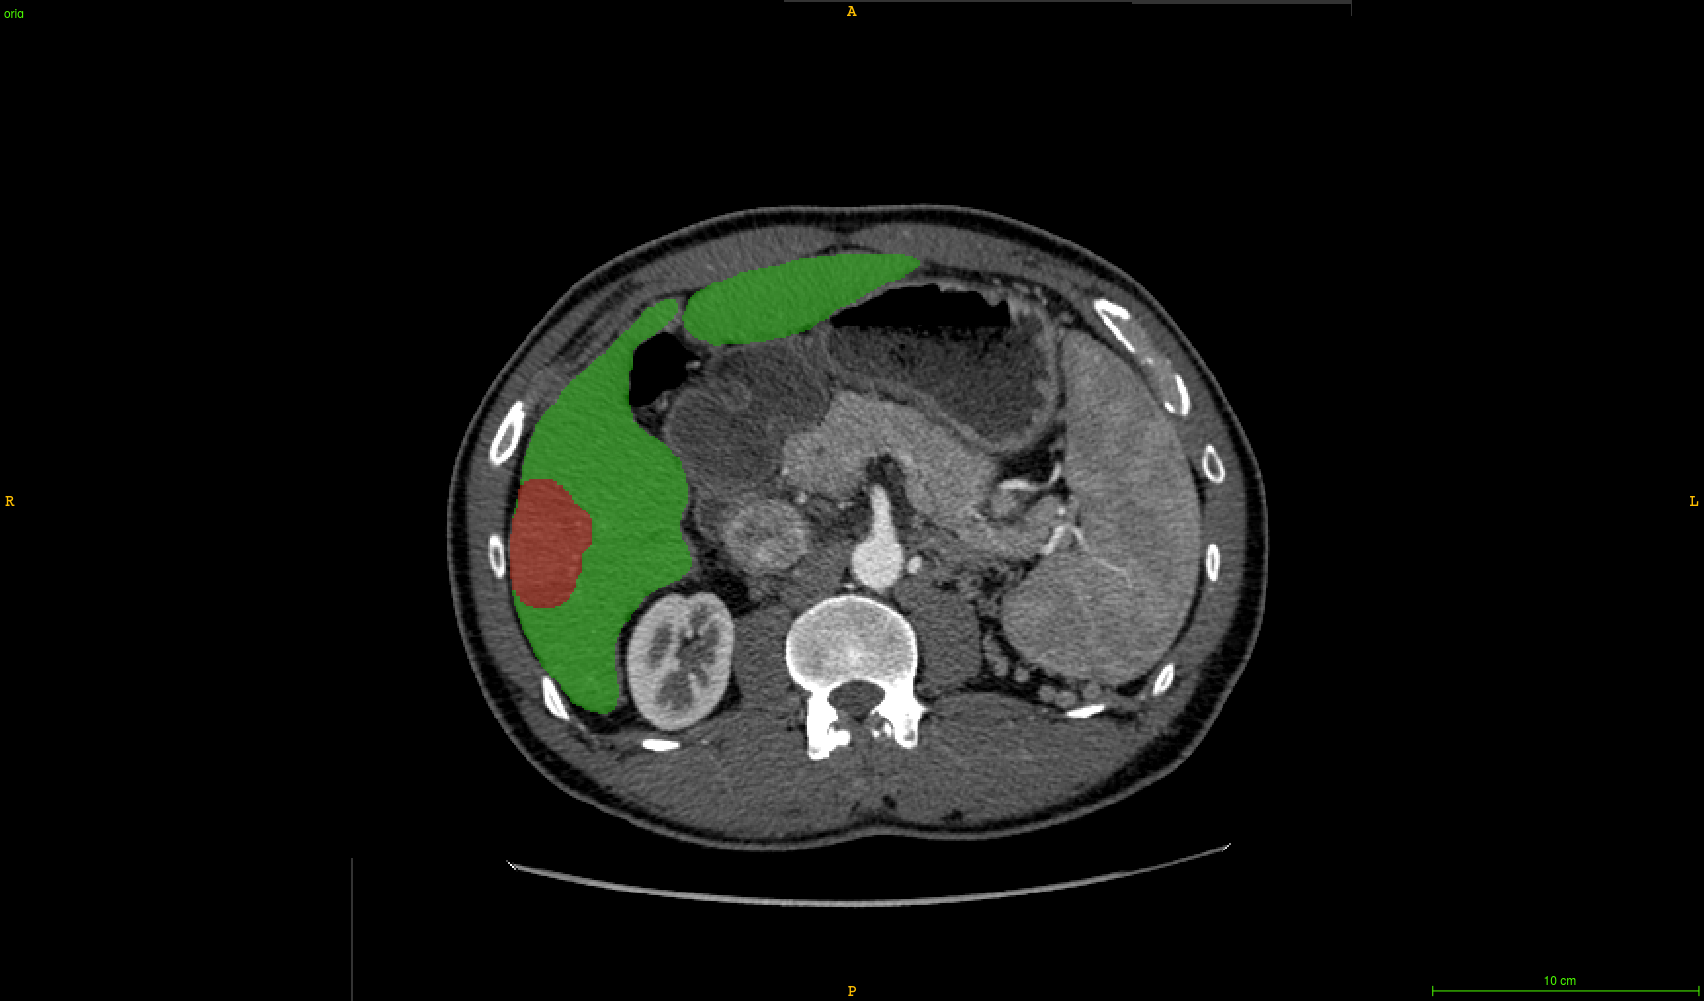
\includegraphics[width=3.10417in,height=3.09722in]{./images/media/image19.png}\tabularnewline
\midrule
\endhead
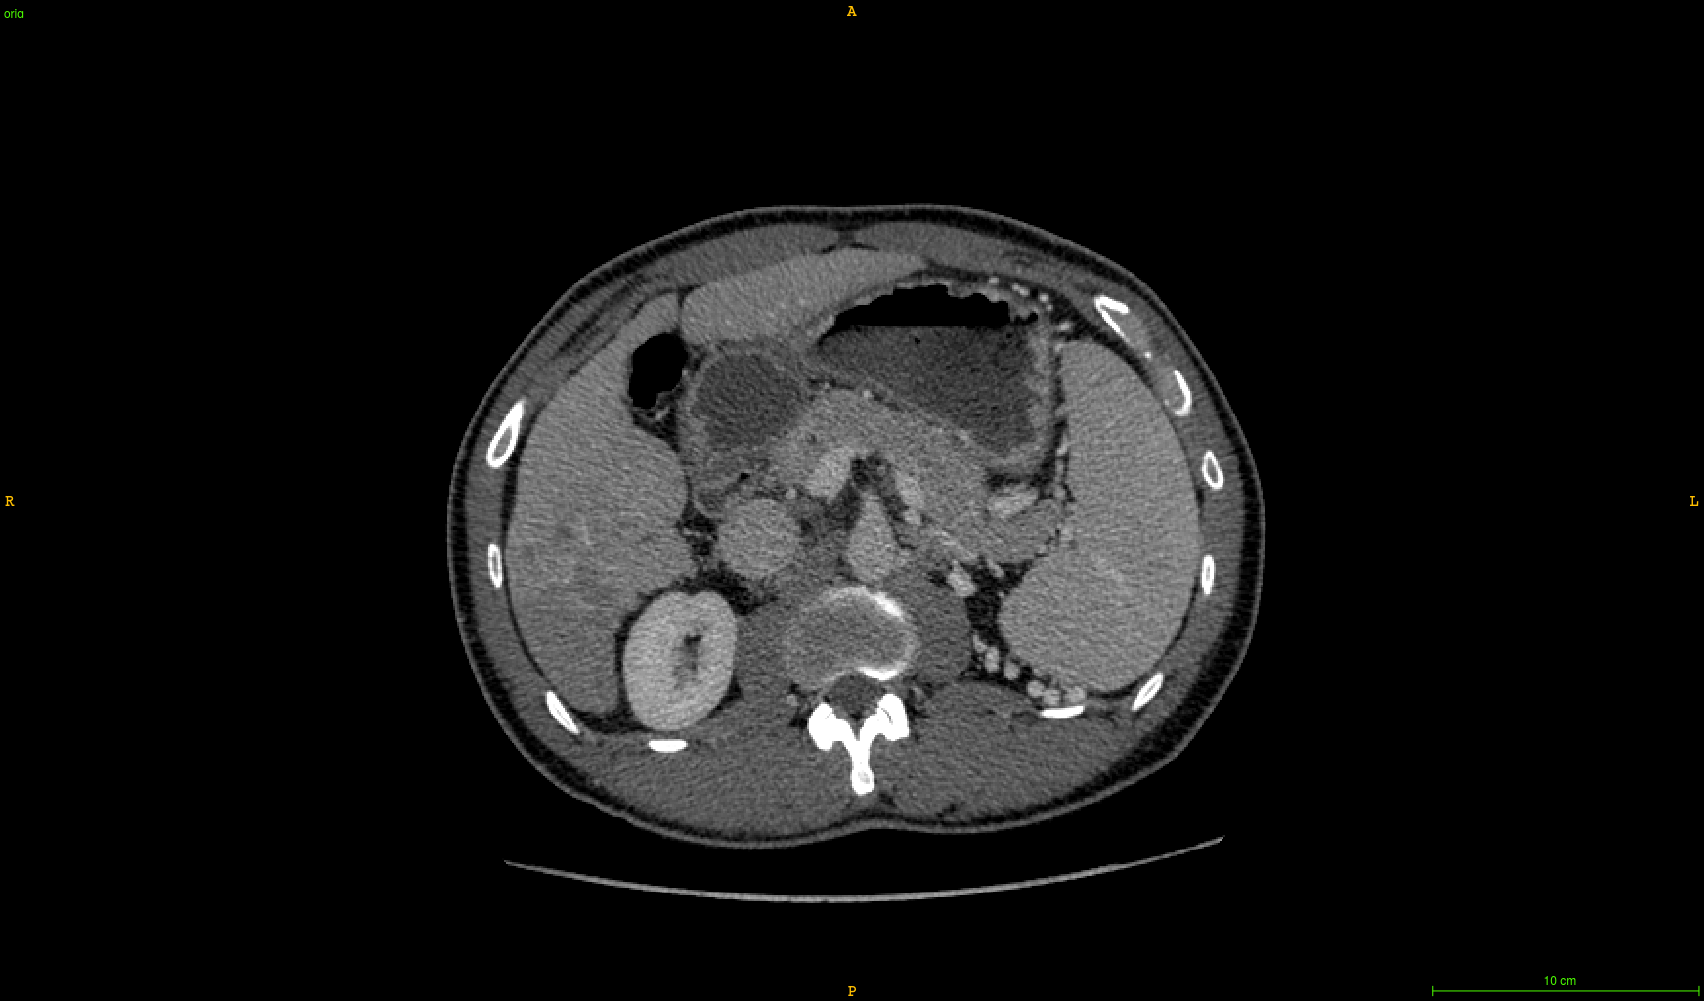
\includegraphics[width=3.10417in,height=3.09722in]{./images/media/image8.png}
&
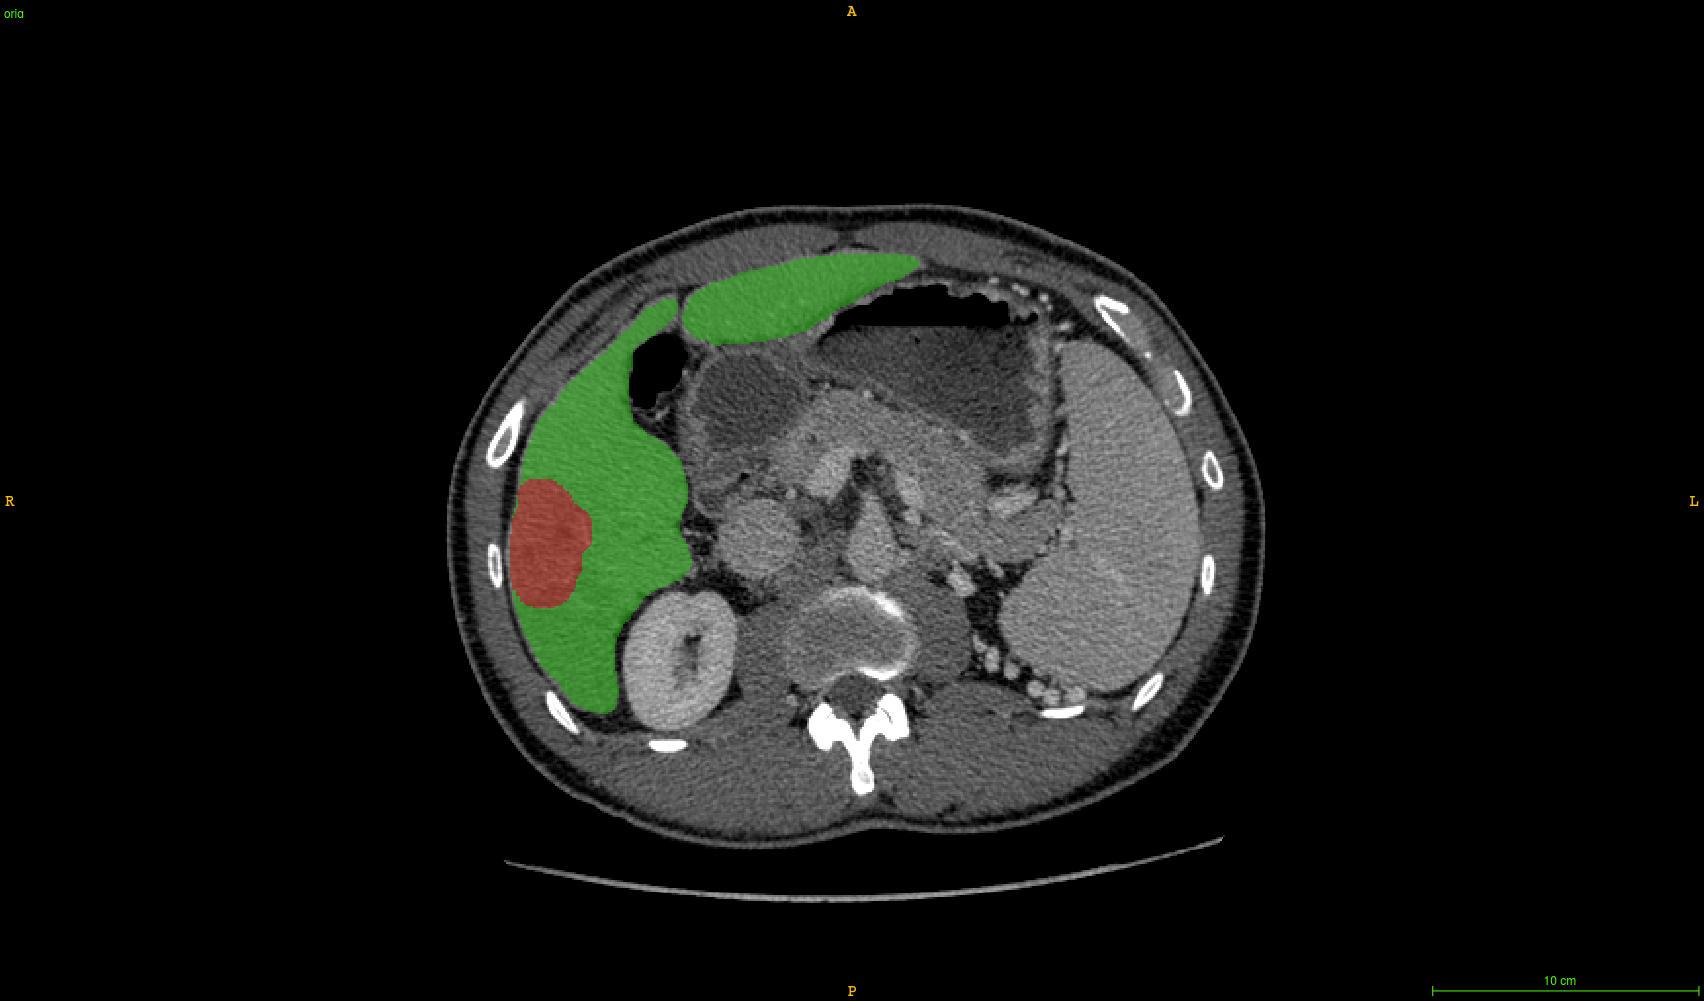
\includegraphics[width=3.10417in,height=3.09722in]{./images/media/image5.png}\tabularnewline
\bottomrule
\end{longtable}

\emph{Example of a patient from G-dB, obtained after enhancing the
dataset with our semantic segmentation network and our registration
pipeline. Top row: AR\_registered volume with original tumor expert
segmentation, bottom row: PV\_volume, left: original raw volumes, right:
segmentation mask overlay where the parenchyma is obtained through our
segmentation pipeline and the tumor was initially delineated by an
expert then transformed to fit the target volume space.}

We were able thanks to our cascaded architecture and a robust liver
segmentation network to enhance the volumes present in G-dB that
originally contained only tumor experts' annotations in AR volumes.

Once a complete database where both the liver and the tumor segmentation
masks were available, and where AR and PV volumes were registered, we
trained a robust multiphase tumor segmentation network.

We trained both a DMP-Tumor and a MPF-Tumor segmentation network on the
registered G-dB dataset, and evaluated them on the TCIA-dB which
contained expert tumor annotations. We evaluated both DMP and MPF
architectures since no statistical differences were available when
comparing results obtained for the tumor segmentation in our previous
work on TheraHCC-dB {[}\textbf{ref CARS}{]}.

We obtained a mean patient-wise DSC of 73.2 +/- 20.6 with MPF
architecture versus 64.9 +/- 27.2 when using the DMP when evaluating the
models on the TCIA-dB patients, after training both architectures with
the same parameters. An example of prediction on the TCIA-dB \textbf{is
depicted in the following figure}.

\begin{longtable}[c]{@{}lll@{}}
\toprule
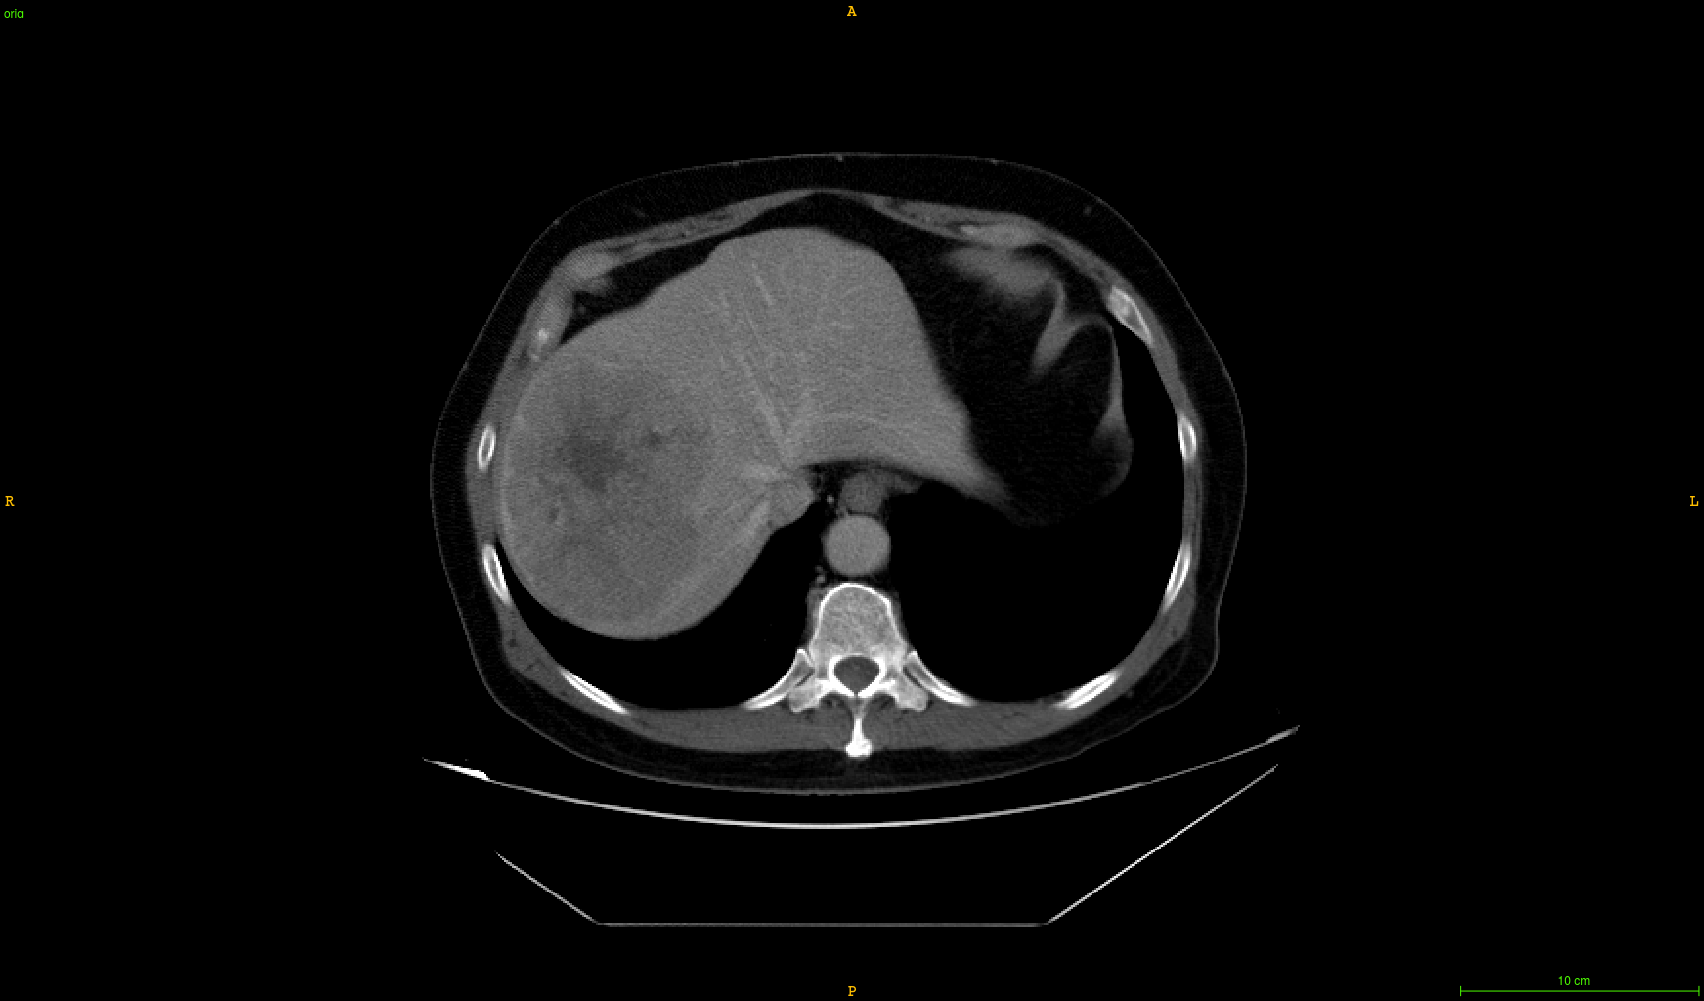
\includegraphics[width=1.94792in,height=1.15278in]{./images/media/image13.png}
&
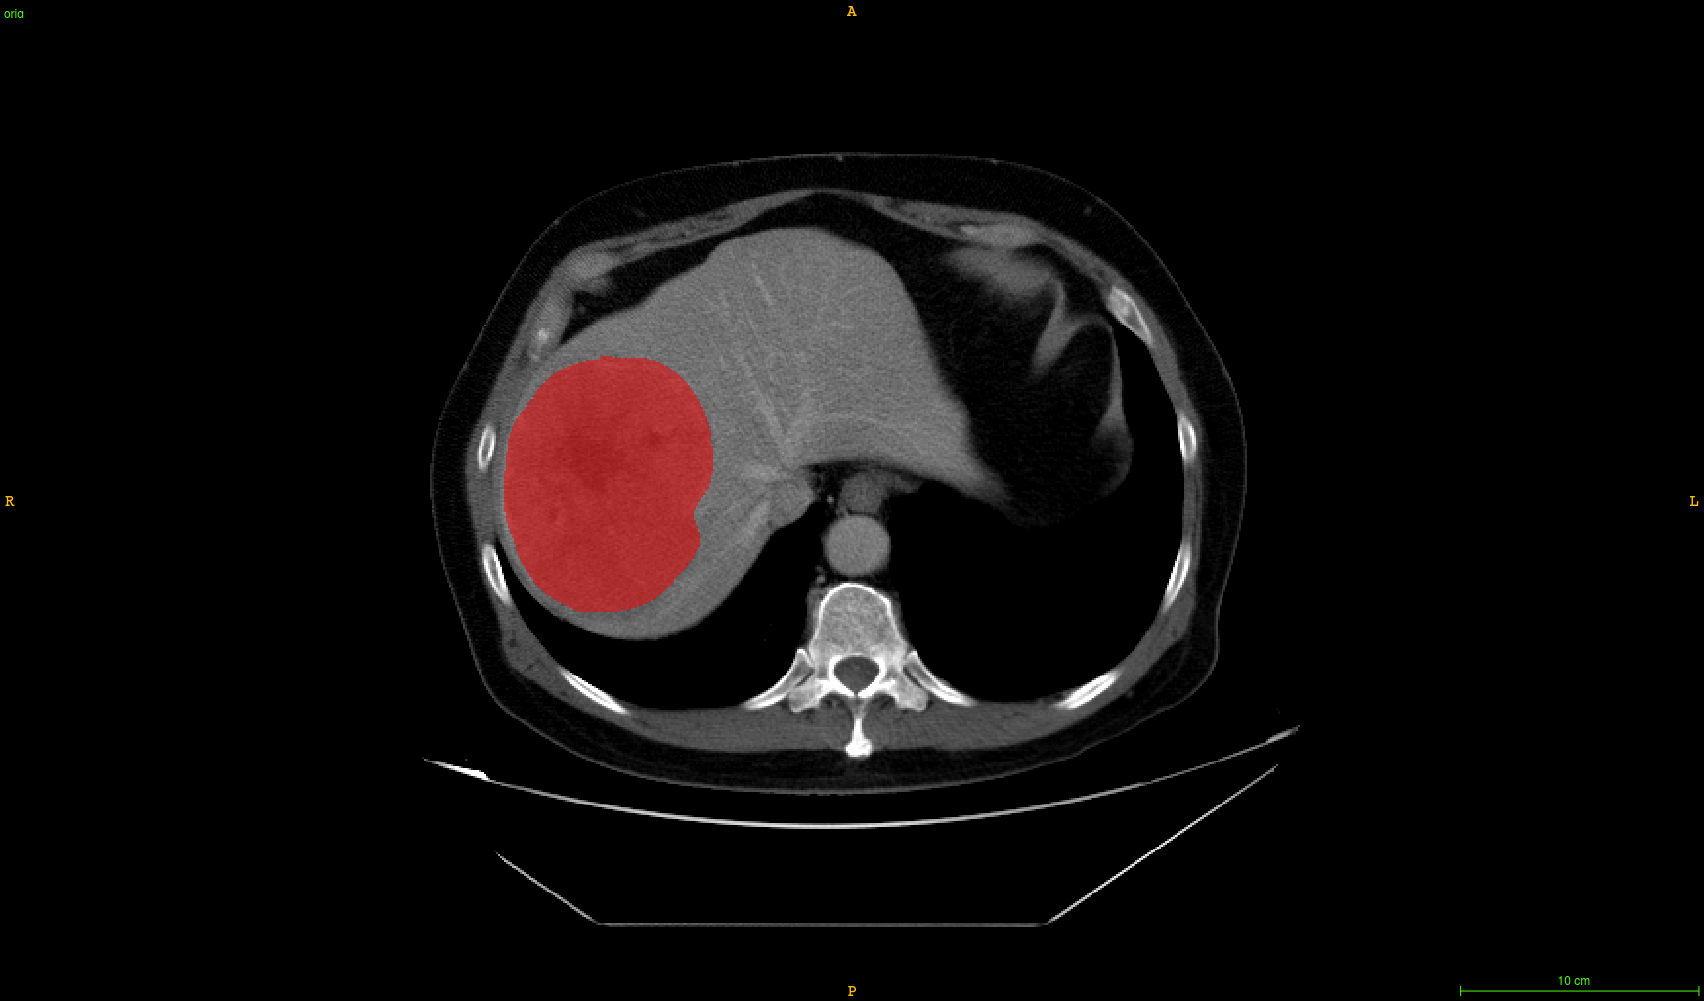
\includegraphics[width=1.94792in,height=1.15278in]{./images/media/image10.png}
&
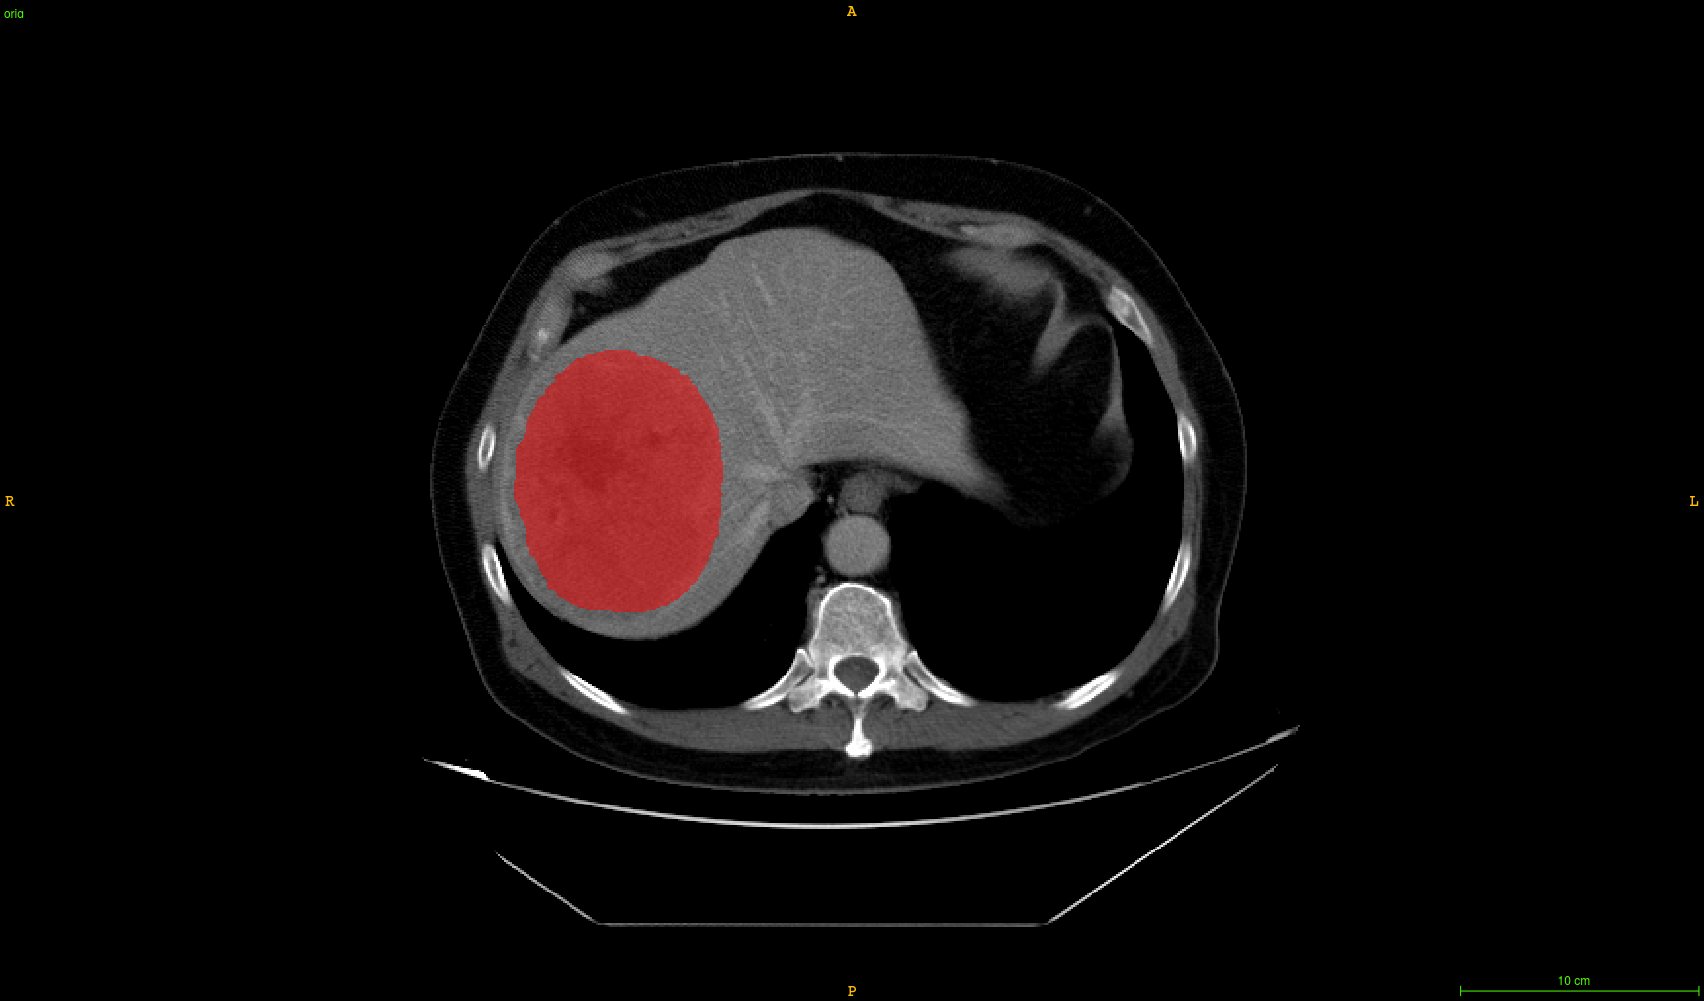
\includegraphics[width=1.94792in,height=1.15278in]{./images/media/image7.png}\tabularnewline
\midrule
\endhead
\bottomrule
\end{longtable}

\emph{\textbf{TODO: change the figure to better see the differences}
Example of an image from the TCIA-dB, with the obtained predicted tumor
segmentation using the MPF-Tumor segmentation network (left: raw,
Middle: expert annotation, right: obtained segmentation)}

Those results obtained on an external dataset tend to show the precision
of the tumor segmentation when training a cascaded architecture with a
sufficient number of cases.

We retained the MPF-Tumor segmentation network since it performed
significantly better than the DMP one (p = 0.02 using a Wilcoxon signed
paired rank test on the patient-wise DSC).

We proved the benefit of the cascaded architecture since those results
were obtained using an architecture where the first network was trained
on LITS-dB and the second was trained on G-dB. We were also able to use
a monophase network for the first step and a multiphasic network for the
second.

This work proved the ability of deep learning (semantic segmentation
network) combined with image processing (registration) to enhance and
complete a weakly annotated database (both TCIA-dB and G-dB were
enhanced in the same way).

Finally, we decided to keep only two stages in our cascaded architecture
since the only available dataset with expert necrosis annotation was the
TheraHCC-dB, containing only 7 patients. This small amount of cases
combined with the aspect of TheraHCC-dB (only sparse slices are
annotated across the volume) might not be enough to precisely
differentiate between the active and the necrotic part of the lesions on
unseen cases. Moreover, the necrosis segmentation appears to be more
sensitive than the tumor segmentation, especially because the necrosis
requires annotations in both phases (in case of AR-PV volumes) since it
can respond differently along the imaging acquisition.

\subsection{Prediction of the histological grade on
TCIA-dB}\label{prediction-of-the-histological-grade-on-tcia-db}

After obtaining the final cascaded architecture, we focused on the
histological grade prediction.

TCIA-dB contains images from 18 patients, where 9 were diagnosed with a
grade 3 (G3), 7 with a grade 2 (G2) and 2 with a grade 1 (G1). In order
to obtain a balanced training dataset, it has been decided to split them
into two groups, the first with G1 and G2 patients, and the second with
G3 patients, as it has been done previously in the literature since G2
was depicted as being closer to G1 than to G3 {[}\textbf{ref 15,16 of
Pawlik}{]}. Patients from the first group (G1 and G2) were considered as
having a low grade, whereas those from the second group have a high
grade.

As explained previously, to train a network dedicated to predict the
histological grade, we have decided to focus on what we called the
relevant imaging semantic features.

We therefore extracted the features from the second network of our
cascaded architecture, to focus on the temporal behavior of the tumor.

The retained network (MPF architecture \textbf{as depicted}
\textbf{previously}) is made of 2 classical U-Net networks, where each
one of them takes either the AR or the PV image as input. We believe
that the compressed information present in the bottleneck part of the
network can be sufficient to encode the total information present in the
network. Therefore, we extracted for each patient of the TCIA-dB, this
encoded information in a slice-wise manner, represented by two 32x32x512
features cube (one per phase in the MPF architecture) per slice
\textbf{as depicted below.}

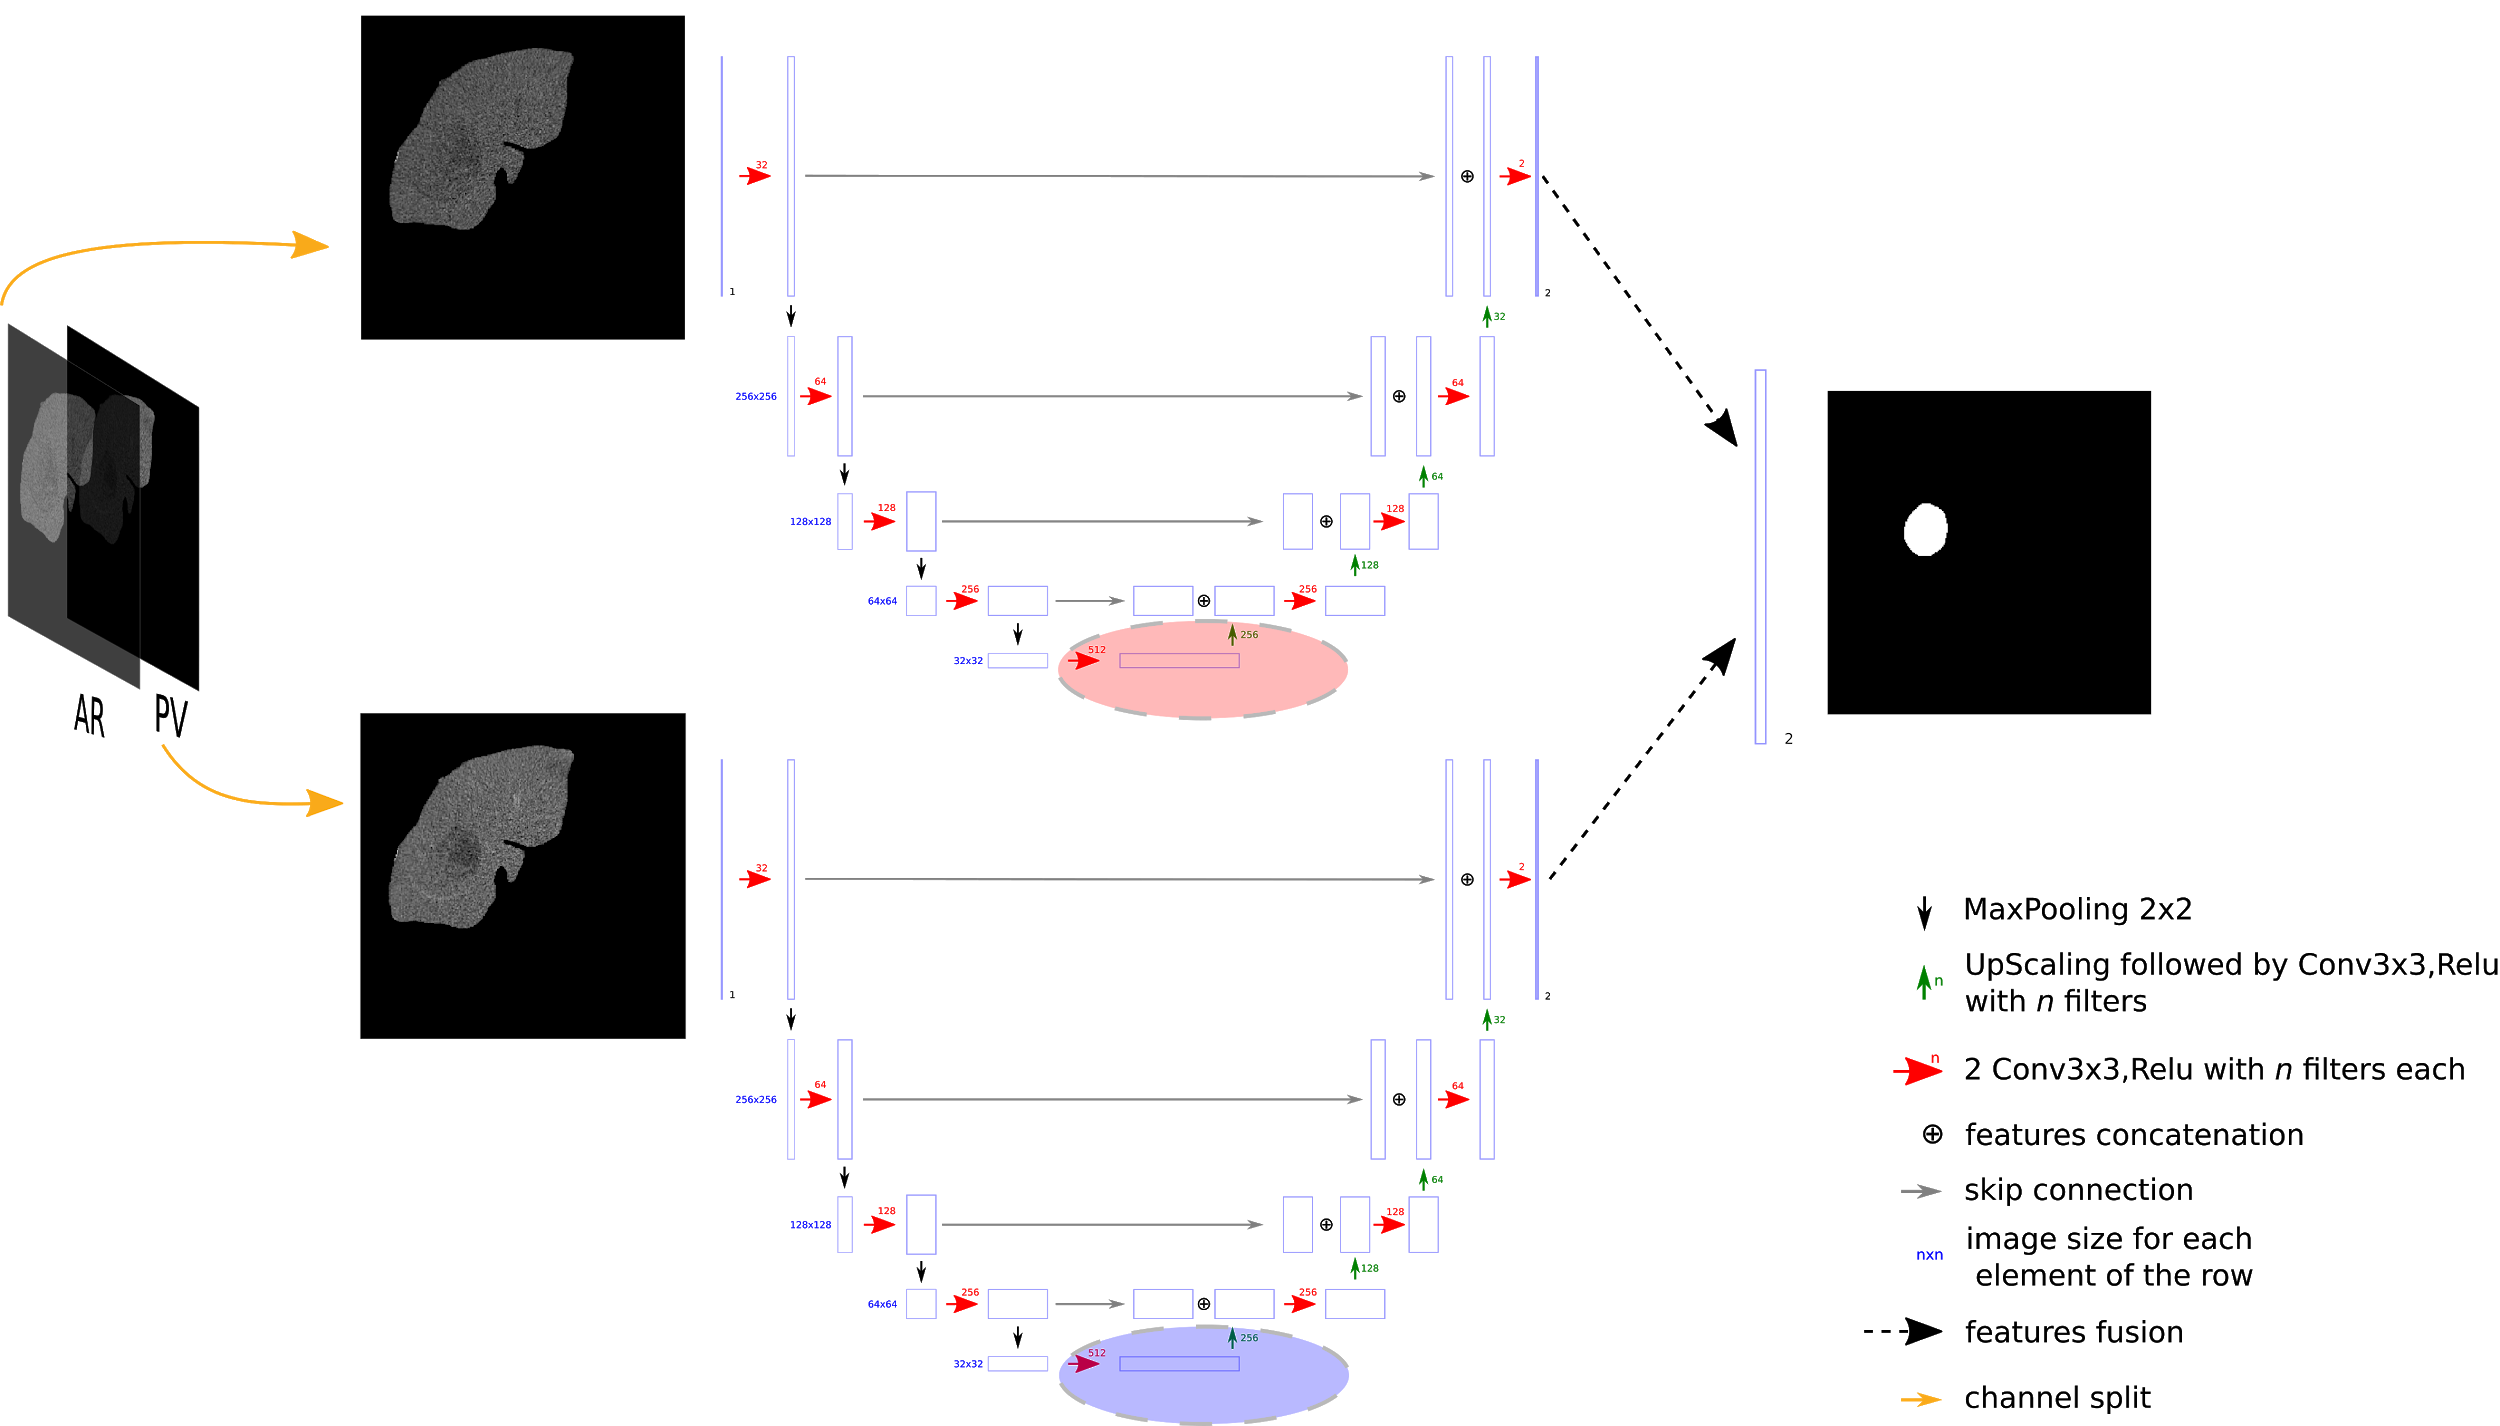
\includegraphics[width=6.26772in,height=3.56944in]{./images/media/image22.png}

\emph{Red and blue areas correspond to the bottleneck part of the U-Net
network where the features extraction is performed. Each image is then
represented as a 32x32x512 features cube.}

Before applying the extraction of the features, we decided to normalize
the dimension of the different volumes of the dataset, so that each
voxel measures 0.68x0.68mm in the axial plane (because it corresponds to
the resolution of the images used to train our semantic segmentation
network), and volumes have a 2.5mm z-spacing (corresponding to the
spacing of the majority of the PV volumes in TCIA-dB).

We finally built an architecture responsible for the grade prediction.
We focused only on the centrally located tumor slices, because the
histological grade corresponds to a measurement of the evolution of the
disease, which tends to have more physiological effects at the center of
the tumor. Centrally located slices will therefore exhibit the highest
grade for a given patient.

Therefore, a slice-wise architecture was built, first because the
features were computed in a slice-wise manner and second because the
histological grade tends to be heterogeneous in the lesion, meaning that
a slice-wise approach allows us to give a finer prediction to find
potential areas with a more advanced disease.

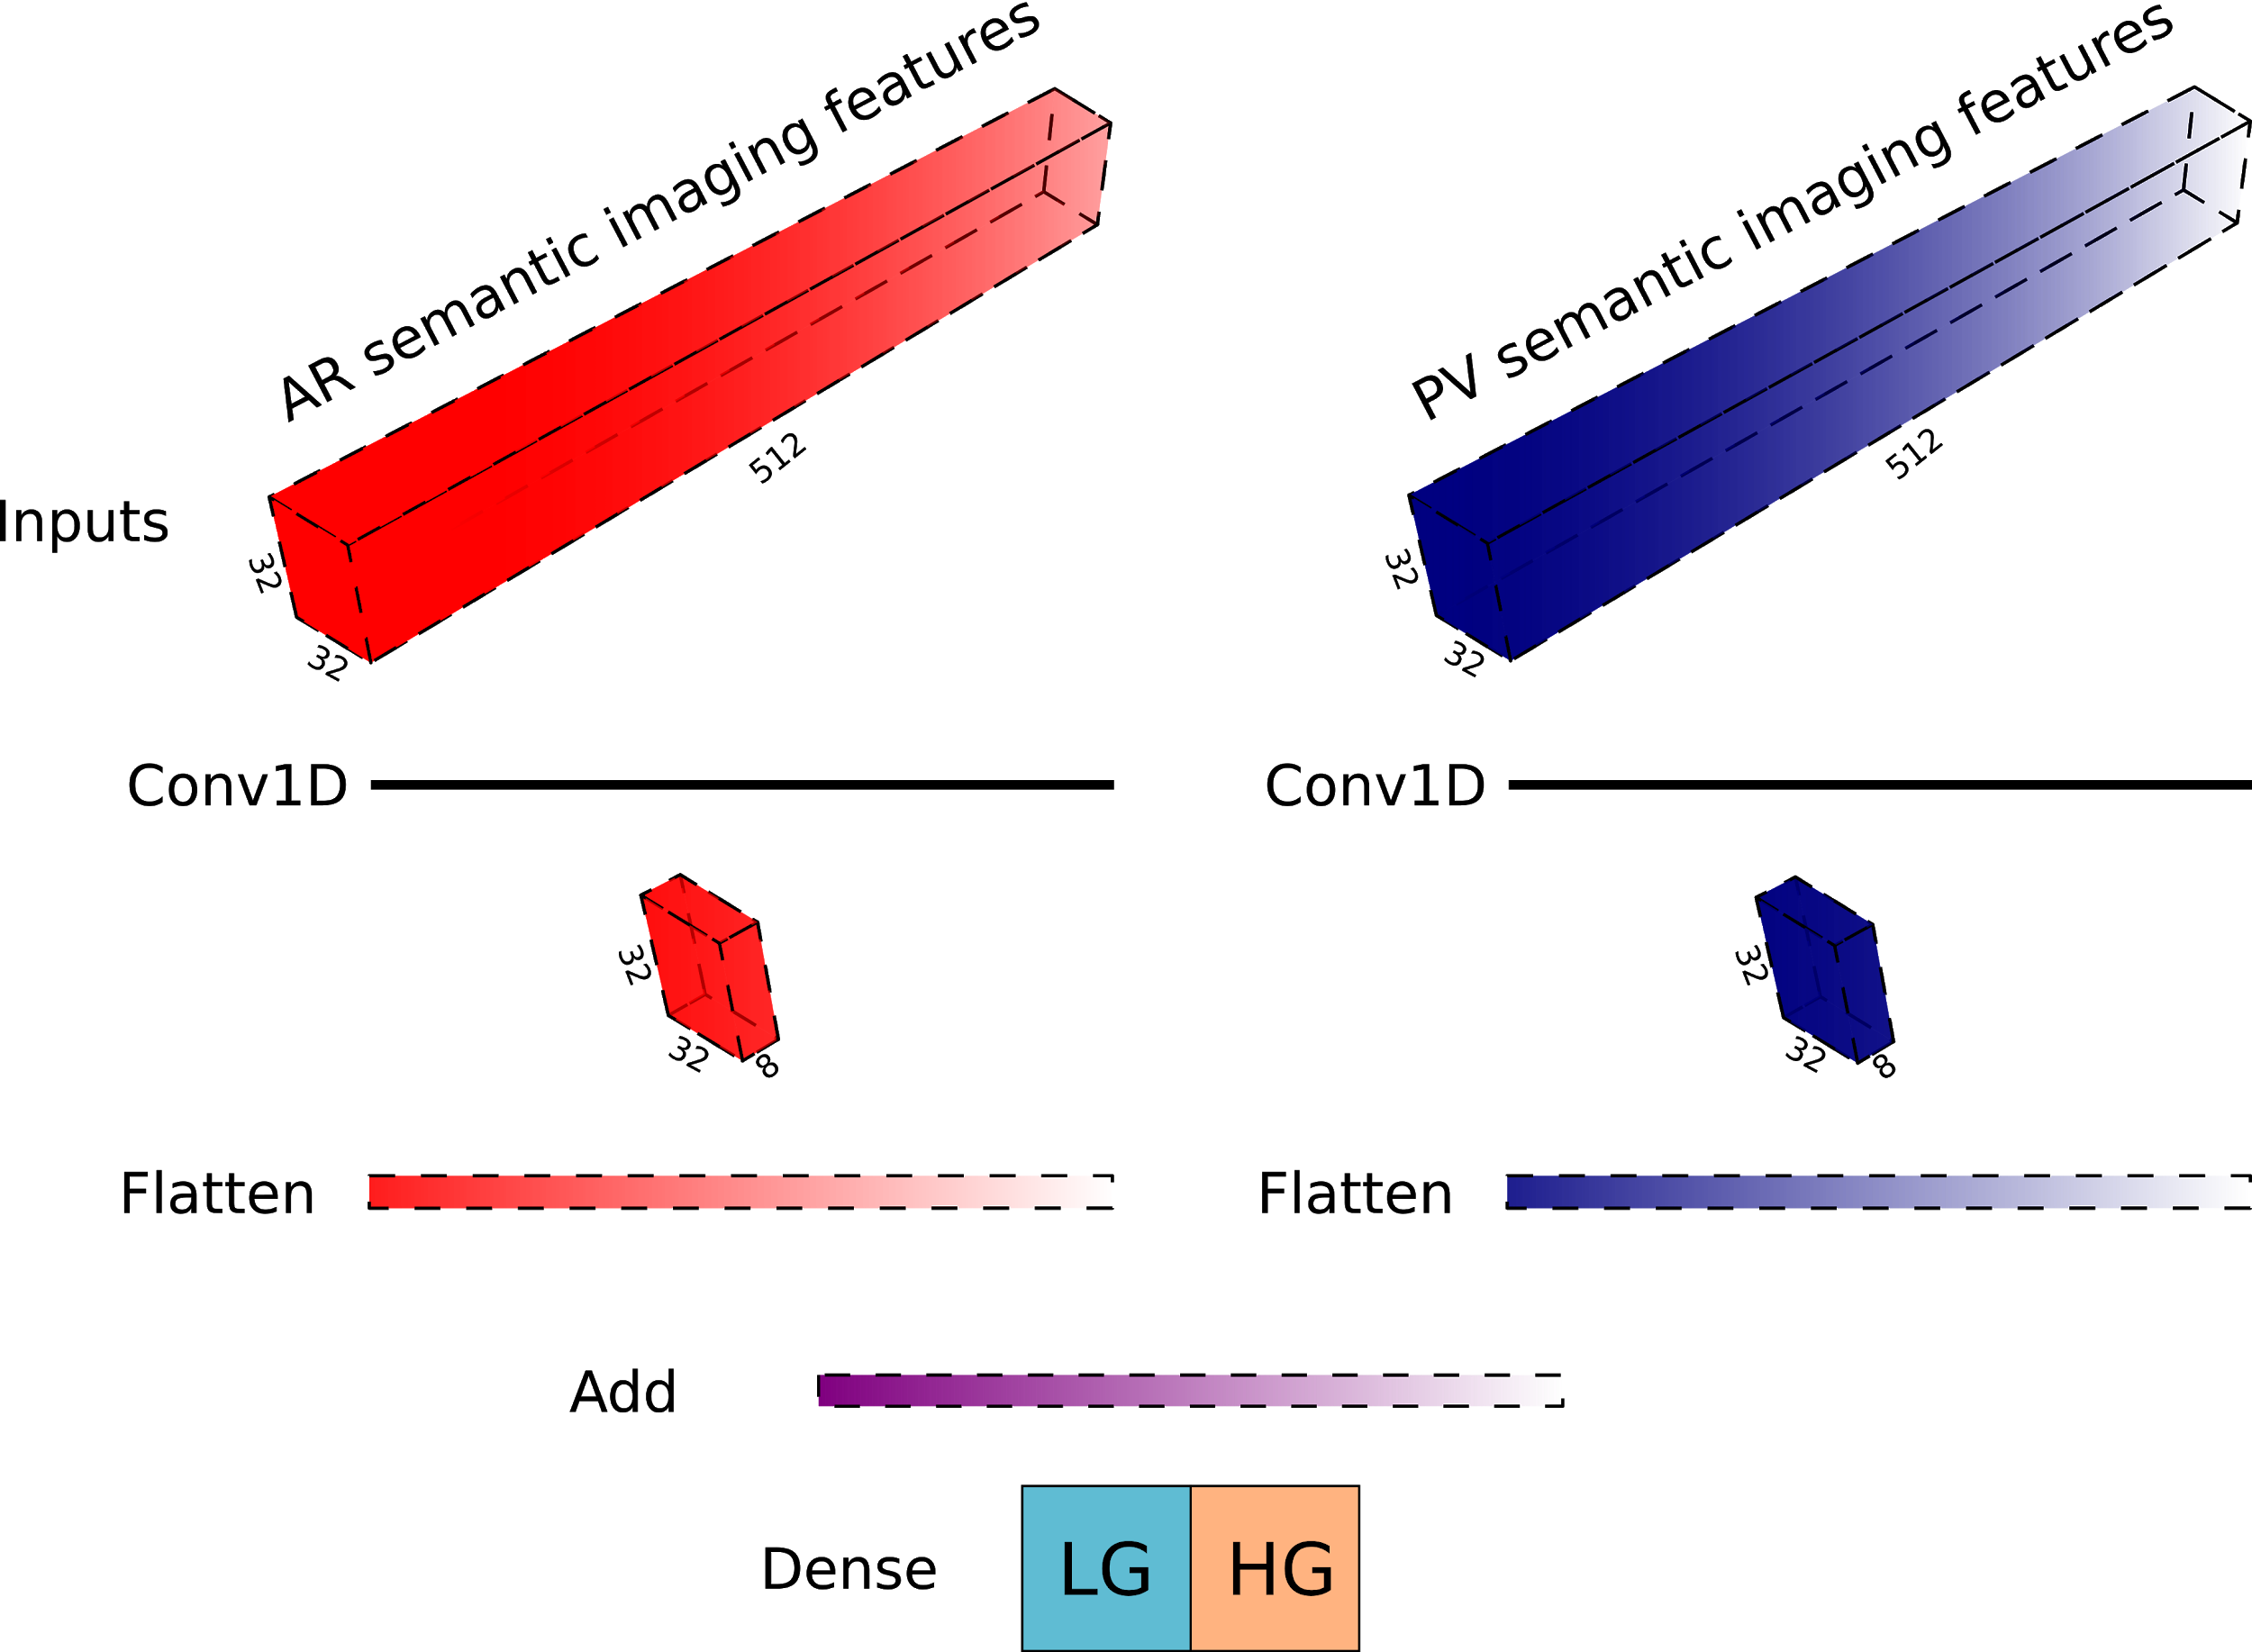
\includegraphics[width=6.26772in,height=4.59722in]{./images/media/image21.png}

\emph{Slice-wise histological grade prediction using both AR and PV
retained semantic imaging features}

The architecture \textbf{depicted above} works as a dimensionality
reduction algorithm, where the first 1D Conv layers are dedicated to
reduce the number of features initially present (32x32x512). The
dimensionality reduction step is performed for both phases separately,
before the remaining features are combined (simple addition in the
features space).

A final dense layer takes the remaining features as input and computes
the probability to belong to each class thanks to softmax activation
function (low vs high grade).

When training the network, we decided to consider that each
centrally-located tumor slice of a given patient will have a higher
probability of exhibiting the highest grade, which in this case
corresponds to the observed patient-wise grade.

Regarding the composition of TCIA-dB (9 high grade patients vs 9 low
grade ones), we performed a 9-fold CV training, so that each patient is
at least present once in the testing set, and so that the training and
the test sets contains both balanced the same number of patients per
class (7 patients from each class in the training set and 1 patient from
each class in the testing set).

After testing several combinations for the hyperparameters, we have
fixed the number of retained features to 8 \textbf{as depicted in the
figure above} (meaning that after the features dimensionality reduction,
we obtained a 32x32x8 cube), and we considered a 2 cm volume
(corresponding to 8 centrally located slices with a 2.5mm spacing) when
training/testing our architecture.

With our CV-training, we were able to correctly predict the patient-wise
histological grade of 15 patients among 18, as detailed in the table
\textbf{hereafter} (a patient is considered as being correctly predicted
when at least half of the retained slices were annotated with the
correct GT class).

When considering a slice-wise prediction, we were able to correctly
predict \textbf{\textasciitilde{}74\%} of the slices.

\begin{longtable}[c]{@{}llll@{}}
\toprule
& & \textbf{True Class} &\tabularnewline
\midrule
\endhead
& & LG & HG\tabularnewline
\textbf{Predicted} & LG & 7 & 1\tabularnewline
& HG & 2 & 8\tabularnewline
& \emph{Total} & 9 & 9\tabularnewline
\bottomrule
\end{longtable}

Those results provided a more detailed prediction than the one
consisting of a single patient-wise classification. Being able to
compute the histological grade locally (here in a slice-wise fashion)
allows us to visually focus on the heterogeneous regions that are
crucial when needing to establish a diagnosis. Our pipeline can also
provide a map of the best biopsy sites that will further be necessary in
the clinical practice to either evaluate the progression of the disease
or its prognosis.

\end{document}
